%%
%% This is file `mcmthesis-demo.tex',
%% generated with the docstrip utility.
%%
%% The original source files were:
%%
%% mcmthesis.dtx  (with options: `demo')
%%
%% -----------------------------------
%%
%% This is a generated file.
%%
%% Copyright (C)
%%       2010 -- 2015 by Zhaoli Wang
%%       2014 -- 2019 by Liam Huang
%%       2019 -- present by latexstudio.net
%%
%% This work may be distributed and/or modified under the
%% conditions of the LaTeX Project Public License, either version 1.3
%% of this license or (at your option) any later version.
%% The latest version of this license is in
%%   http://www.latex-project.org/lppl.txt
%% and version 1.3 or later is part of all distributions of LaTeX
%% version 2005/12/01 or later.
%%
%% This work has the LPPL maintenance status `maintained'.
%%
%% The Current Maintainer of this work is latexstudio.net.
%%
%%
%% This is file `mcmthesis-demo.tex',
%% generated with the docstrip utility.
%%
%% The original source files were:
%%
%% mcmthesis.dtx  (with options: `demo')
%%
%% -----------------------------------
%%
%% This is a generated file.
%%
%% Copyright (C)
%%       2010 -- 2015 by Zhaoli Wang
%%       2014 -- 2019 by Liam Huang
%%       2019 -- present by latexstudio.net
%%
%% This work may be distributed and/or modified under the
%% conditions of the LaTeX Project Public License, either version 1.3
%% of this license or (at your option) any later version.
%% The latest version of this license is in
%%   http://www.latex-project.org/lppl.txt
%% and version 1.3 or later is part of all distributions of LaTeX
%% version 2005/12/01 or later.
%%
%% This work has the LPPL maintenance status `maintained'.
%%
%% The Current Maintainer of this work is Liam Huang.
%%

\documentclass{mcmthesis}
\mcmsetup{CTeX = false,   % 使用 CTeX 套装时,设置为 true
        tcn = 2207690, problem = C,
        sheet = true, titleinsheet = true, keywordsinsheet = true,
        titlepage = false, abstract = true}
% \usepackage{newtxtext}%\usepackage{palatino}
\usepackage{tikz}
\usepackage{lipsum}
\usepackage{algorithm}
\usepackage{algorithmicx}
\usepackage{algpseudocode}
\usepackage{amsmath}
\usepackage{graphicx} %插入图片的宏包
\usepackage{float} %设置图片浮动位置的宏包
\renewcommand{\algorithmicrequire}{\textbf{Input:}}
\renewcommand{\algorithmicensure}{\textbf{Output:}} % Use Output in the format of Algorithm
\title{End-to-end Reinforcement Learning-Based Novel Portfolio Management Model}
\author{\small \href{MCM 2022 Team 2207690}
  {\includegraphics[width=7cm]{mcmthesis-logo}}}
\date{\today}
\begin{document}

\begin{abstract}
% Use this template to begin typing the first page (summary page) of your electronic report. This template uses a 12-point Times New Roman font. Submit your paper as an Adobe PDF electronic file (e.g. 1111111.pdf), typed in English, with a readable font of at least 12-point type.

% Do not include the name of your school, advisor, or team members on this or any page.

% Papers must be within the 25 page limit.

% Be sure to change the control number and problem choice above.
% You may delete these instructions as you begin to type your report here.

% Follow us @COMAPMath on Twitter or COMAPCHINAOFFICIAL on Weibo for the most up to date contest information.

Portfolio management is the process of managing investments,
constantly rearranging a certain amount of funds into several products or assets,
aiming at maximizing profit and ensuring minimizing risks at the same time.

This article presents a portfolio management model based on end-to-end reinforcement learning, using the proximal policy optimization(PPO).
Also, other multi-staged methods are used as a comparison, including RNN-LSTM (i.e. Recurrent Neural Network with Long Short-Term Memory) and the vector autoregressive model.

The article proposes a method to control trading risk artificially, introducing the market risk premium.
It is used to control the maximum amount of risk that can be accepted in each transaction as a way of adjusting the relationship between return and risk.

All the methods are examined with the data given, during the five-year trading period from 9/11/2016 to 9/10/2021.
The learning result shows that the PPO with high risk constraint gained the most, by a factor of 112.

\begin{keywords}
Portfolio arrangement; Vector autoregressive model; Reinforcement learning;
\end{keywords}
\end{abstract}
\maketitle

\tableofcontents
\newpage

\section{Introduction}
\subsection{Background of the problem}

 Investment in financial products is a common way to produce extra income and favorable profits.
This means the buy and sell of several products at a time,
which can be rather relatively stable ones such as national debt,
or volatile assets, for example, gold and bitcoin.
While investing can make profits, it can also carry certain risks,
especially when the product is relatively unstable.
To maximize the profit and minimize the risk of an investment,
traders usually invest in several products at a time
and decide the holdings of each asset based on actual market conditions.
In terminology, this method is called \textit{portfolio management}.

Portfolio management is the process of managing investments,
constantly rearranging a certain amount of funds into several products or assets,
aiming at maximizing profit and ensuring low market risks at the same time\cite{jiang2017deep}.
There have been several traditional methods to solve this problem,
which can be roughly classified into these four categories\cite{li2014online}:

\begin{itemize}
  \item \textbf{Follow the winner}\\
  maximize the portfolio's expected growth rate
  \item \textbf{Follow the loser}\\
  transfer the fund from \textit{winner} asset to \textit{loser} asset
  \item \textbf{Pattern Matching}\\
  predict future market distribution based on historical data
  \item \textbf{Meta-Learning}
\end{itemize}

There're many algorithms that combine these methods with machine learning.
These algorithms are reliable in short-term prediction
but do not behave well in long-term prediction.
This is because the algorithms highly depend on their accuracy,
but the natural uncertainty of the market makes it hard to predict.

\subsection{Restatement of the problem}

Based on the historical gold and BTC price data,
develop a model that helps to determine the holdings of cash, gold, and bitcoin every single day.
To note, the daily trading strategy should only be made using the price data before that day.

The final target is to make maximum profit from the given 1,000 USD principal,
and predict how much it will become five years later, based on the formerly developed model.

% \subsection{Syntax (how to type \LaTeX\ commands --- these
%   are the rules)}

% \lipsum[3]
% \begin{itemize}
% \item the angular velocity of the bat,
% \item the velocity of the ball, and
% \item the position of impact along the bat.
% \end{itemize}
% \lipsum[4]
% \emph{center of percussion} [Brody 1986], \lipsum[5]

% \begin{Theorem} \label{thm:latex}
% \LaTeX
% \end{Theorem}
% \begin{Lemma} \label{thm:tex}
% \TeX .
% \end{Lemma}
% \begin{proof}
% The proof of theorem.
% \end{proof}

% \subsection{Other Assumptions}
% \lipsum[6]
% \begin{itemize}
% \item
% \item
% \item
% \item
% \end{itemize}

% \lipsum[7]

\section{Analysis of the Problem}



% \subsection{Transaction Costs}

% % 然而,在实际的市场中,往往不能忽略交易的手续费。在考虑手续费时,设计的投资策略必须有效预计未来资产价格的走势情况,如果在短时间内频繁交易,由于手续费的存在,整体盈利会被极大影响。

% However, in the actual market, the transaction cost cannot be ignored. When considering the transaction cost, the designed investment strategy must effectively predict the future trend of asset prices. If there are frequent transactions in a short period of time, the overall profit will be greatly affected due to the existence of the transaction cost.

% % 在现实中,Transaction cost通常来自于资产佣金,交易市场等机构会在交易时收取阶梯定价的手续费,这些手续费通常与买卖资产的市值正相关。这种自然的手续费是无法被正确衡量的。然而,我们的模型做了一些简单化的假设,假定手续费是按照资产交易的数额按照百分率收取的,并且买入和卖出的手续费一致。

% In reality, transaction costs usually come from asset commissions. Institutions such as trading markets will charge tiered pricing fees during transactions. These fees are usually positively related to the market value of assets bought and sold. This natural fee cannot be measured correctly. However, our model makes some simplistic assumptions, assuming that fees are charged as a percentage of the amount traded on the asset, and that the fees for buying and selling are the same.

\section{Hypotheses}

\begin{itemize}
  \item \textbf{Market closure days}\\
  There are cases that data is missing in the gold price data given.
  It can be observed that this vacancy basically occurs on weekends
  and during holidays such as Christmas day and the days around.
  We assume such vacancies occur on and only on gold market closure days.
  In this case, gold cannot be traded and the gold price won't change.\\
  This does not apply for the bitcoin market, which does not have closure days.
  \item \textbf{Trade at the end of the day}\\
  Price changes during the trading hours each day are not taken into consideration
  as there is no relevant data.
  We assume that the data given in the question is the \textit{closing price}
  (i.e. the price at the end of the trading hours),
  and our trade is made at that market closing time ideally.
  \item \textbf{Transaction Costs}\\
  Transaction cost is a factor that cannot be ignored. If frequent transactions are done in a short period of time, the overall profit will be greatly affected due to the existence of the transaction cost.\\
  In actual markets, transaction costs usually come from asset commissions. Institutions such as trading markets will charge tiered pricing fees during transactions. These fees are usually positively related to the market value of assets bought and sold. This natural fee cannot be measured correctly. However, our model makes some simplistic assumptions, assuming that fees are charged as a percentage of the amount traded on the asset, and that the fees for buying and selling are the same.
  \item \textbf{Ignore market impact}\\
  The amount of funds we put into the market is very little
  compared to the total assets in the market.
  Thus, we assume that our actions have zero effect on the market itself.
  \item \textbf{Instant trading}\\
  Transactions in the market are fast enough to be considered immediate.
  This allows us to take out or put in money once we make a trade, with no delay.
\end{itemize}

% \begin{figure}[h]
% \small
% \centering
% \includegraphics[width=8cm]{example-image-a}
% \caption{The name of figure} \label{fig:aa}
% \end{figure}

% \lipsum[8] \eqref{aa}
% \begin{equation}
% a^2 \label{aa}
% \end{equation}

% \[
%   \begin{pmatrix}{*{20}c}
%   {a_{11} } & {a_{12} } & {a_{13} }  \\
%   {a_{21} } & {a_{22} } & {a_{23} }  \\
%   {a_{31} } & {a_{32} } & {a_{33} }  \\
%   \end{pmatrix}
%   = \frac{{Opposite}}{{Hypotenuse}}\cos ^{ - 1} \theta \arcsin \theta
% \]
% \lipsum[9]

% \[
%   p_{j}=\begin{cases} 0,&\text{if $j$ is odd}\\
%   r!\,(-1)^{j/2},&\text{if $j$ is even}
%   \end{cases}
% \]

% \lipsum[10]

% \[
%   \arcsin \theta  =
%   \mathop{{\int\!\!\!\!\!\int\!\!\!\!\!\int}\mkern-31.2mu
%   \bigodot}\limits_\varphi
%   {\mathop {\lim }\limits_{x \to \infty } \frac{{n!}}{{r!\left( {n - r}
%   \right)!}}} \eqno (1)
% \]

\section{The two-staged methods}

\subsection{Introduction}

% It is a general approach to make regressing from past price dates and forecasting a period price. Then design an algorithm to make a plan for rearranging the ratio of assets. These methods can be classified as ``two-staged methods''.
The workflow of a two-staged method can be roughly summarized into two steps:

\begin{itemize}
  \item Make regressing from past price dates and forecasting a period price;
  \item Design an algorithm to make a plan for rearranging the ratio of assets.
\end{itemize}

In the prediction stage, there are mainly two methods in the industry, namely Vector Autoregression (VAR) and LSTM.

The first method, vector autoregression model, is a highly recognized time series analysis model. In previous research, vector autoregression model has been widely used in investment management, quantitative trading and so on. These models usually model the existing data, and then select the last piece of data for prediction and comparison as a reference. The autoregressive model has been shown to have very good interpolation accuracy and can also accurately predict the development trend in the next few days in terms of prediction.

As for the second method, we try to use the recurrent neural network method to train the processed data. However, if we only use the recurrent neural network, the model we build will be unable to deal with the exponential explosion or gradient of the weights caused by the recursion. It is difficult to obtain the data changes of bitcoin and gold value in a long period of time due to the disappearance of the problem, so on the basis of using the recurrent neural network, we use the long short-term memory network to optimize, so that the neural network The time points covered by the model are further advanced, extending the memory of the network. The RNN-LSTM model is very common and its code is open source. Thus, we built the network and predicted the data through the open source deep learning library.

We use the bitcoin price data to train our models, with the last seven days of data as the test set and other data as the training set. Our model will predict the last 7 days of price of bitcoin, then use these price data to compare with the actual price to judge whether the prediction is reasonable.
The prediction results of the autoregressive model will be shown in figure\ref{fig:prediction} together with the prediction results of the RNN-TLSM model and the workflow of the prediction model is shown in figure \ref{AR}.

\begin{figure}[h]
  \tikzset{every picture/.style={line width=0.75pt}} %set default line width to 0.75pt

  \begin{tikzpicture}[x=0.75pt,y=0.75pt,yscale=-1,xscale=1]
  %uncomment if require: \path (0,300); %set diagram left start at 0, and has height of 300

  %Straight Lines [id:da8112233976325808]
  \draw    (100,101) -- (544,101) ;
  \draw [shift={(546,101)}, rotate = 180] [color={rgb, 255:red, 0; green, 0; blue, 0 }  ][line width=0.75]    (10.93,-3.29) .. controls (6.95,-1.4) and (3.31,-0.3) .. (0,0) .. controls (3.31,0.3) and (6.95,1.4) .. (10.93,3.29)   ;
  %Straight Lines [id:da7920278133084296]
  \draw    (512,65) -- (512,137) ;
  %Curve Lines [id:da46433491372617774]
  \draw    (265,124) .. controls (255.1,176.47) and (360.85,241.68) .. (401.78,213.87) ;
  \draw [shift={(403,213)}, rotate = 143.13] [color={rgb, 255:red, 0; green, 0; blue, 0 }  ][line width=0.75]    (10.93,-3.29) .. controls (6.95,-1.4) and (3.31,-0.3) .. (0,0) .. controls (3.31,0.3) and (6.95,1.4) .. (10.93,3.29)   ;
  %Curve Lines [id:da102775317135267]
  \draw    (566,208) .. controls (605.8,178.15) and (637.68,116.62) .. (571.01,88.42) ;
  \draw [shift={(570,88)}, rotate = 22.38] [color={rgb, 255:red, 0; green, 0; blue, 0 }  ][line width=0.75]    (10.93,-3.29) .. controls (6.95,-1.4) and (3.31,-0.3) .. (0,0) .. controls (3.31,0.3) and (6.95,1.4) .. (10.93,3.29)   ;

  % Text Node
  \draw (519,70) node [anchor=north west][inner sep=0.75pt]   [align=left] {7 days};
  % Text Node
  \draw (245,74) node [anchor=north west][inner sep=0.75pt]   [align=left] {Training data};
  % Text Node
  \draw (411,195) node [anchor=north west][inner sep=0.75pt]   [align=left] {Prediction Model};
  % Text Node
  \draw (551,157) node [anchor=north west][inner sep=0.75pt]   [align=left] {predict};

  \end{tikzpicture}

  \caption{A workflow of the prediction model}
  \label{AR}
\end{figure}

Next topic, we will focus on the process of building an autoregressive model.


\subsection{Establishment of the autoregressive model}

Before we start building the autoregressive model, the correlation coefficient must be determined. If the correlation coefficient is not high enough, the autoregressive model cannot be solved.

\subsubsection{Determine whether the data is stationary}
The autoregressive model can only be applied to predict economic phenomena related to its own previous period (also known as its data stationary/weak stationary), such as economic phenomena that are greatly affected by its own historical factors, the mining volume of mines, the output of various natural resources etc.For economic phenomena that are greatly affected by social factors, autoregressive models are not suitable. Therefore, before establishing an autoregressive model, we first need to judge whether the subject conditions meet the requirements for establishing an autoregressive model.

First of all, formulate the null hypothesis $H_0$ :
\[
 H_0 : \mbox{Here is a unit root/UNIT ROOT}
\]
% 存在单位根/UNIT ROOT(即数据不平稳)
% 自回归模型只能适用于预测与自身前期相关的经济现象(也称作其数据平稳/弱平稳),例如受到自身历史因素影响较大的经济现象,如矿的开采量,各种自然资源产量等;对于受到社会因素影响较大的经济现象,不宜采用自回归模型。因此,在建立自回归模型之前,我们首先需要判断一下题目条件是否符合自回归模型的建立要求

The next step is to do hypothesis testing.
In existing statistics we can do it with \textit{Augmented Dickey-Fuller Test}(ADF test), which is always used to identify whether there is a single root in the sample data of individual variables in time series analysis.
By using ADF test, we can get the following results(three decimal places):

\begin{table}[h]
  \centering
  \begin{tabular}{@{}lr@{}}
    \toprule
    Name & Value \\
    \midrule
    Statistical values & -0.238 \\
    P-value & 0.934 \\
    lags & 24.000 \\
    nobs & 1801.000 \\
    Threshold value(1\%) & -3.434 \\
    Threshold value(5\%) & -2.863 \\
    Threshold value(10\%) & -2.568 \\
    \bottomrule
  \end{tabular}
  \caption{ADF test result}
\end{table}


In the form, \textit{Statistical values}, \textit{P-value} and \textit{lags} are all statistical values obtained under the AIC standard, and the first parameter is used for comparison with the lower 1\%, 5\%, and 10\% cutoffs.
The second parameter represents the probability that the null hypothesis holds.
The parameter \textit{nobs} is the number of observations used in this detection.
The parameter maxlag in \textit{ADF TEST} is determined by it, and the formula is $ \displaystyle maxlag = 12 \times ( \frac{nobs}{100}) ^\frac{1}{4} $ .

It can be seen from the \textit{P-value} that the probability of the null hypothesis is extremely low, thus we can reject the null hypothesis $H_0$, and the data is stationary.
% 由p值可以看出,原假设成立的概率极底,我们应该拒绝原假设。即数据平稳

\subsubsection{Quickly see if the data fits the AR model}
  According to the autoregressive function:

  \begin{equation}
    \hat{y_t} = b_0 + b_1 \times y_{t - 1} + \ldots + b_n \times y_{t - n}, \qquad n < t
  \end{equation}

  We can determine whether $ y_{t + 1}$ and $ y_t $ are clearly related from figure \ref{fig:lag_plot}. Also, we can calculate that the correlation coefficient is 0.998 and the significance level is 0.0, approximately.

  \begin{figure}[h]
    \centering
    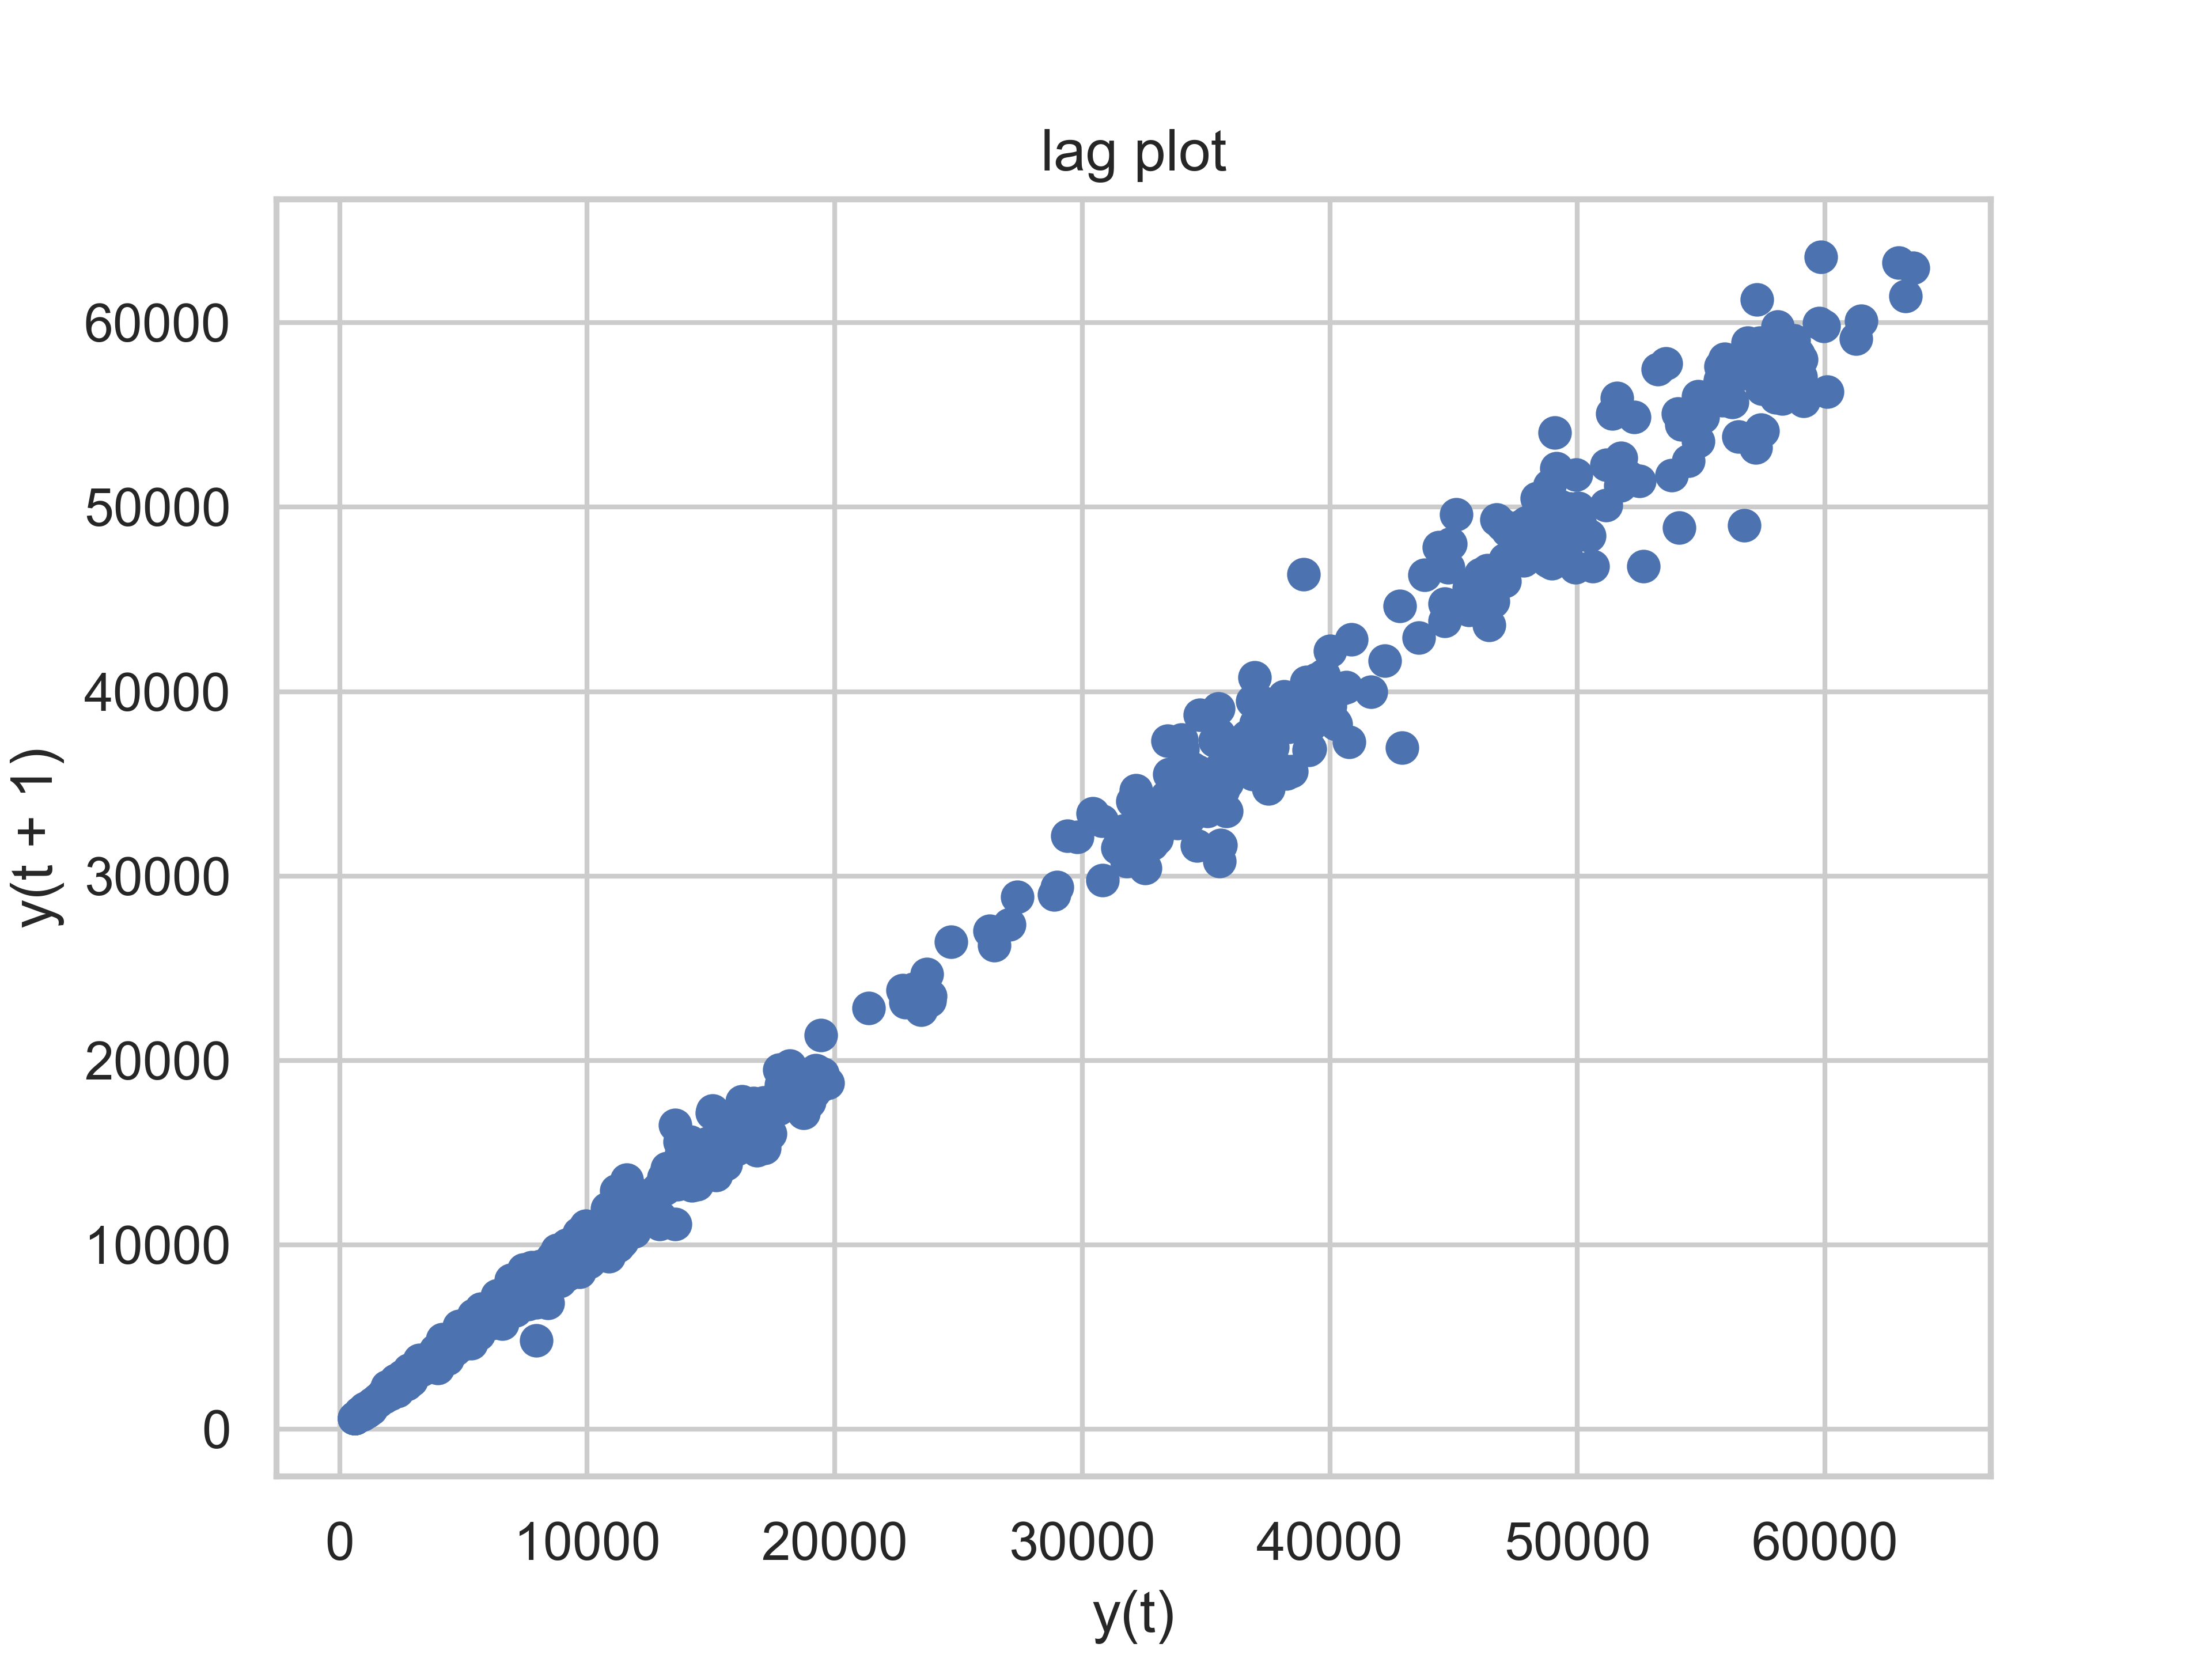
\includegraphics[width=0.5\textwidth]{lag_plot}
    \caption{The lag plot of correlation}
    \label{fig:lag_plot}
  \end{figure}

  When we judge the correlation of $ y_t$ and $ y_{t - 1} \ldots y_{t - n} $ at the same time, we plot the autoregressive coefficients of n multiple lags at a time, as shown in the figure \ref{fig:correlation}.

  \begin{figure}[h]
    \centering
    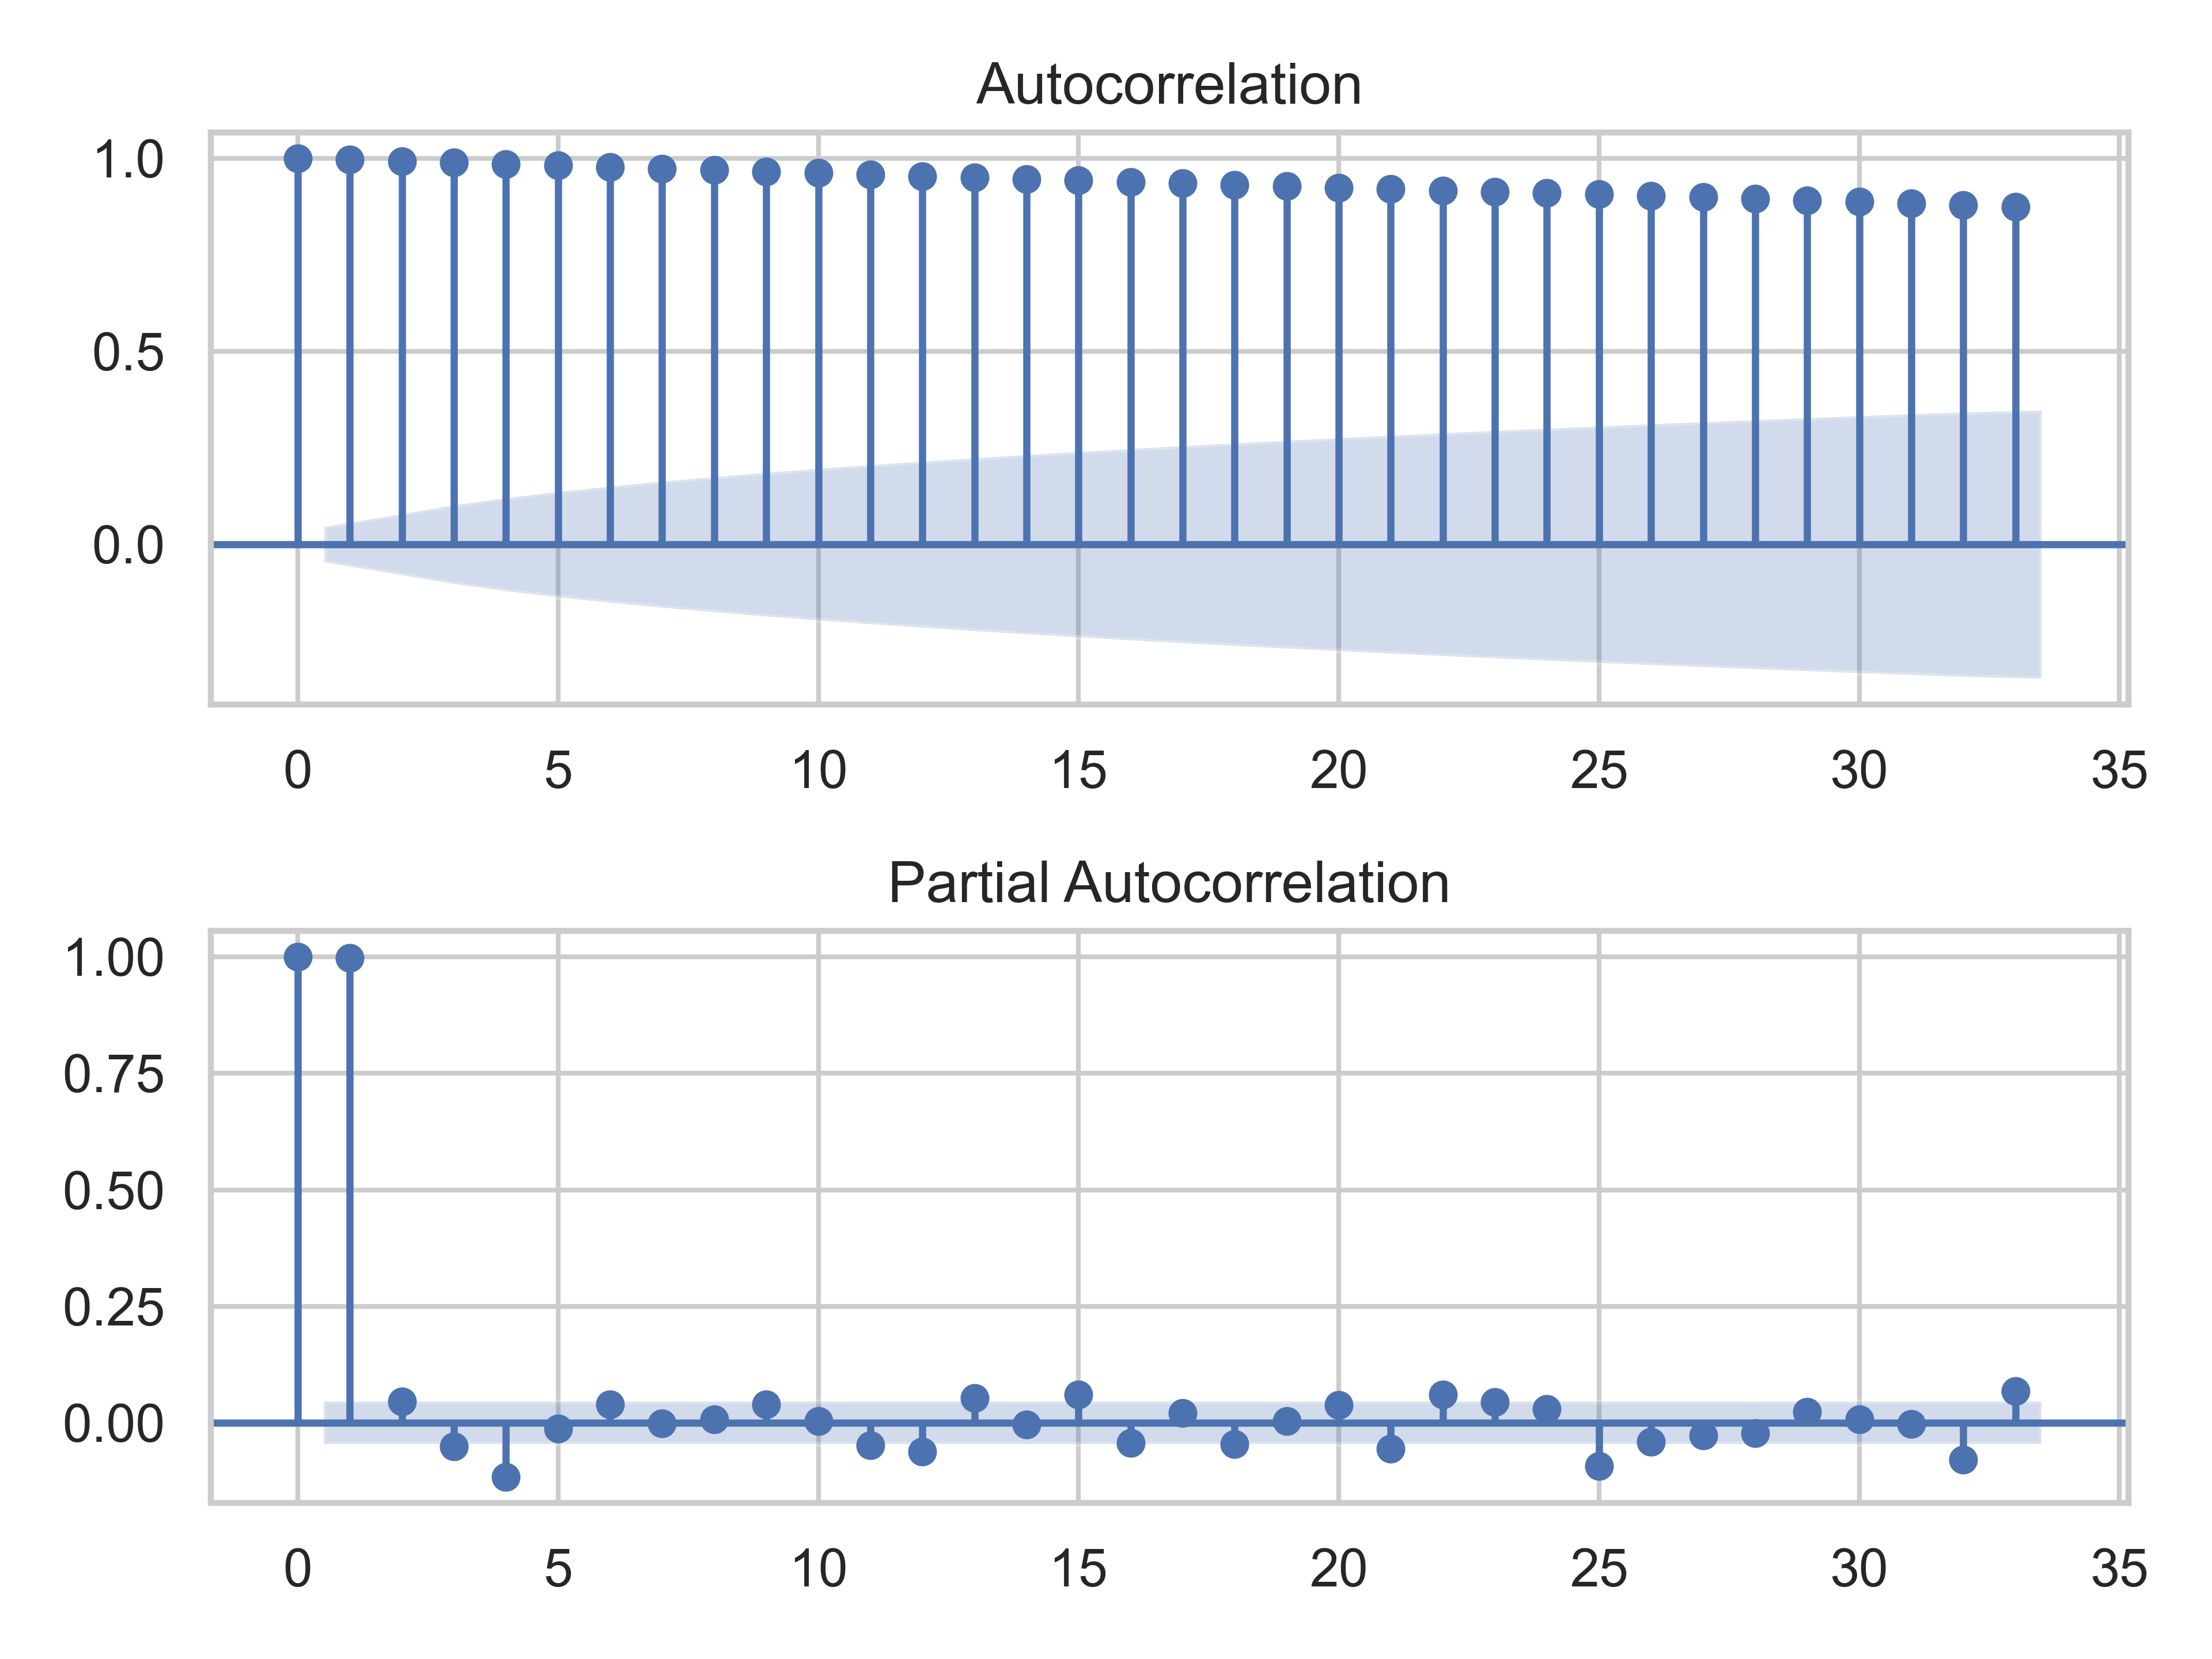
\includegraphics[width=0.5\textwidth]{correlation}
    \caption{Multiple autoregressive coefficients}
    \label{fig:correlation}
  \end{figure}

\subsubsection{Build the training model}
We use the data except the last seven days to train our model and compare the predicted data for the last seven days with the real data provided in the table, and the results are shown in figure \ref{fig:prediction}.

\begin{figure}[h]
  \centering
  \includegraphics[width=0.5\textwidth]{3_result}
  \caption{Comparison of predicted results}
  \label{fig:prediction}
\end{figure}
\subsection{Model summary}

% 两阶段的模型通常依赖于在第一阶段准确的预测,而第二阶段的规划则相对不那么重要且原始。这直接导致两阶段模型通常较为“短视”他们不能根据长期增长情况作出长远规划。

Two-stage models typically rely on accurate predictions in the first stage, while planning in the second stage is relatively less important and primitive. In addition, both models have a certain lag in time, and this leads directly to the fact that two-stage models are often ``short-sighted''. Thus, they cannot make long-term plans based on long-term growth.

However, the performance of an algorithm capable of planning a portfolio based on predictions obtained from any two-staged model depends on the accuracy of the model's predictions to a large extent, and it is obvious that the future market prices are too complex to predict accurately. Also, if we translate the price predictions, which are not market behavior actually, into actions, we have to build an additional layer of logic.If we establish a neural model on this base, then we can no longer take transaction cost into account.In this case of manual coding, we can not consider the method as reliable fully machine learning.As a result we turned to trying to apply reinforcement learning to make predictions on the data.Compared with supervised learning that can only consider one-time problems, focus on short-term benefits and consider immediate rewards, reinforcement learning has a more long-term perspective, considering long-term rewards and can find optimal solutions to many problems. Furthermore, the reinforcement learning approach we present below shows a more general ability to consider transaction costs as one of the important risks.

% 我们的工作将使用这些two-staged方法作为对照实验,评估我们更优化的模型的performance。

% Our work will use these two-staged methods as control experiments to evaluate the performance of our more optimized models.


\section{Reinforcement learning model}

As concluded before,
the method of predicting with VAR is straightforward to think of,
but still not accurate enough.
Thus, this section presents a possible solution using the Reinforcement learning (RL) model, one of the one-staged methods,
trying to improve the algorithm accuracy.

\subsection{Introduction to reinforcement learning}

\subsubsection{One-staged methods}

Compared to two-staged methods, a one-staged method is end-to-end, which means it directly arrange its actions from the past data, skipping the processes between the input and the output\cite{lecun2004autonomous}.
In a multi-staged method, a task is solved in multiple steps, where the input to each step is the output of the previous step.
This can cause accumulation of inaccuracy which may be exponential as the number of steps increases in the worst case.
One-staged methods eliminate the influence between different steps and reduces the complexity of the algorithm.

\subsubsection{Deep learning}

Deep learning is part of machine learning and also part of artificial intelligence,
based on artificial neural networks, or ANN.
ANN is inspired by the biological neural network
and shares a similar structure with it, as diagram \ref{ANN} shows:

\begin{figure}[h]
\small
\centering
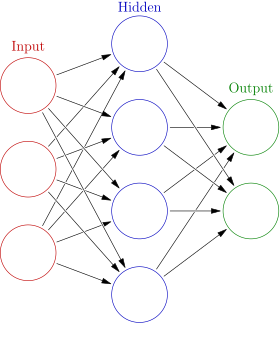
\includegraphics[width=5cm]{Colored_neural_network.svg.png}
\caption{Artificial neural network} \label{ANN}
\end{figure}

An ANN is based on a collection of connected units or nodes called artificial neurons,
which corresponds to the concept of neurons in a biological brain.
The connections between these nodes are called \textit{edges}.
They can transmit signals from one node to another,
just like what synapses in a biological brain do.
Inside each node, the data from the previous node is calculated in a non-linear way
and passed on to the next node.

The 'deep' in deep learning refers to the use of multiple layers in ANN.
Nodes in ANN are divided into several layers,
and different layers might perform different transformations on the input data.
The very first layer is called the input layer and,
accordingly, the last layer is referred to as the output layer.
Those layers between the first and the last layer are called \textit{hidden} layers.

Deep learning can be divided into three categories.
The learning is rather supervised, semi-supervised, or unsupervised.
Every neuron and edge has a \textit{weight} that can be adjusted in the learning process.
Given sample \textit{observations}, ANN adjusts the weight of the nodes and edges,
trying to improve the accuracy of the output.
This process is done by lowering the observed error rate.
In this case, learning won't stop until
extra observations don't efficiently reduce the error rate.

\subsubsection{Reinforcement learning}

 Reinforcement learning is a field of deep learning.
Diagram \ref{LA} shows the basic elements of reinforcement learning:

\begin{figure}[h]
  \small
  \centering
  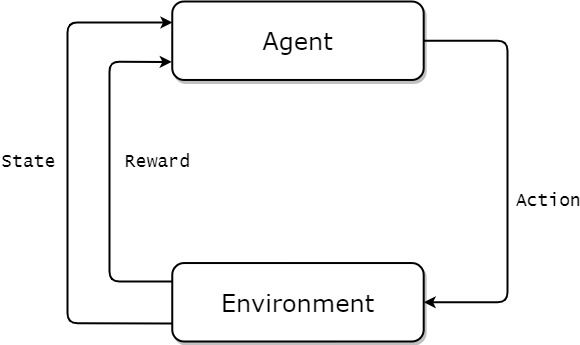
\includegraphics[width=9cm]{RL.jpg}
  \caption{Reinforcement learning} \label{LA}
\end{figure}

In a reinforcement learning model, there is one \textit{agent},
who performs as a learner or decision-maker.
\textit{Actions} of the agent influences the \textit{environment}.
In turn, the environment determines the \textit{state} of the learner
and gives the learner a certain amount of \textit{reward}.
It's kinda like a game, where players take their actions and get a relevant award from the system.
Players will continuously change their actions to maximize their rewards.

A reinforcement learning model works just like that,
but there are no game guides it can refer to --
all given to the model is some ``in-game data''.
Reinforcement learning does not require a large quantity of data to feed,
as supervised learning and unsupervised learning do.
Briefly, reinforcement learning is a ``trial and error'' approach to learning,
interacting constantly with the environment to gain feedback and
adjust behavior for maximum reward.

\subsubsection{Markov decision process}

 The process studied by deep learning is usually normalized as a \textit{Markov decision process}, or MDP.
MDPs are defined to have \textit{Markov property}:

\begin{itemize}
  \item The future can be fully predicted only using \textit{present} states;
  \item The future does not depend on the \textit{past};
  \item The past does not \textit{directly} effect the future.
\end{itemize}

In one word, Markov property refers to the memoryless property of a process, or

\begin{equation}
  P(s_{t+1}\vert s_t) = P(s_{t+1}\vert s_t,...,s_2,s_1).
\end{equation}

A stochastic and continuous decision-making process with Markov property
is called a Markov decision process.
An MDP can be described as a 4-tuple:

\begin{equation}
(\pmb{S},\pmb{A},\pmb{P},\pmb{R})
\end{equation}

\begin{itemize}
  \item $\pmb{S}$ is the set of states, called the state space;
  \item $\pmb{A}$ is the set of actions, called the action space;
  \item $\pmb{P}_a(s_t, s_{t+1})$ is the probability that action $a$ in state $s_t$ on day $t$ will lead to state $s_{t+1}$ on day $t+1$;
  \item $\pmb{R}_a(s_t, s_{t+1})$ is the expected reward received on day $t+1$, based on state $s_t$ and action $a$ on day $t$.
\end{itemize}

These elements make the foundation of MDPs.
A simplified MDP is shown in diagram \ref{MDP}.

\begin{figure}[h]
  \small
  \centering
  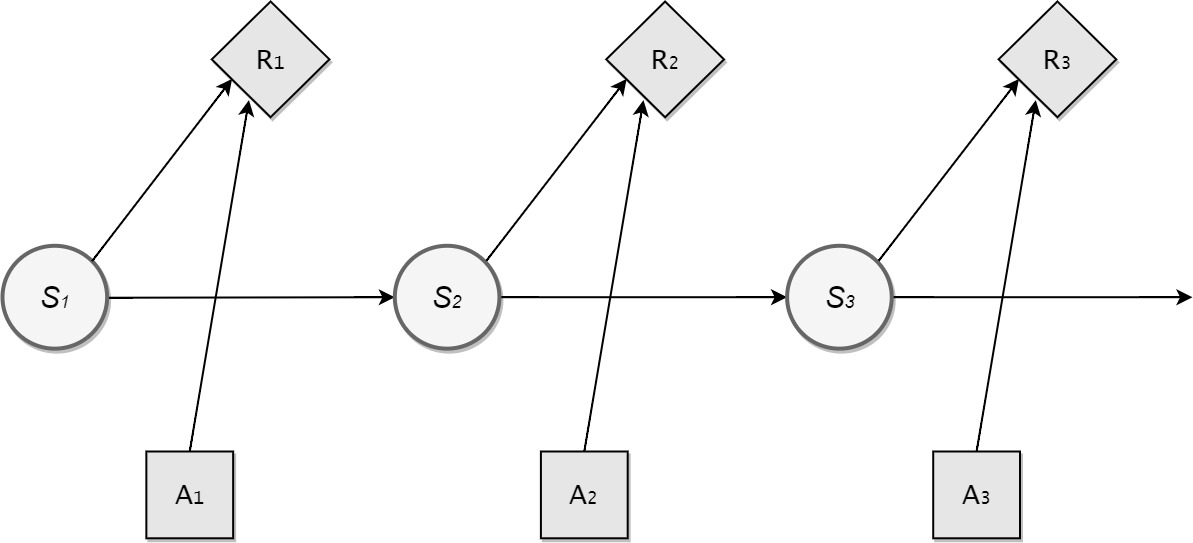
\includegraphics[width=11cm]{MDP.jpg}
  \caption{Markov decision process} \label{MDP}
\end{figure}

With all these $\pmb{A}$s and $\pmb{R}$s,
the goal is abstracted as finding an exact way to decide all the $a_t$
to maximize the final reward.
This reward is the combination of all the $\pmb{R}$s.
In most cases, it represents the mathematical expectation of the sum of $\pmb{R}$s,
$E(\Sigma R)$.

\subsubsection{Proximal policy optimization}

Proximal policy optimization (PPO) is a policy gradient method for reinforcement learning.

Here, we use PPO to interact with the environment and update policy $\pi_\theta(a_t | s_t)$ hrough a clipped surrogate function $L^{CLIP}$. Assuming that

\[
r_t(\theta) = \frac{\pi_{\theta}(a_t | s_t)}{\pi_{\theta_{\mathrm{old}}}(a_t | s_t)}
\]

and we let

\[
  L^{CLIP}(\theta) = \hat{\mathbb{E}}_t \left[ \min \left(r_t(\theta) \hat{A}_t, \mathrm{clip}(r_t(\theta), 1 - \epsilon, 1 + \epsilon)\right) \hat{A}_t \right]
\]

Where $\epsilon$ is a hyperparameter, generally set to $\epsilon = 0.2$ , and then use SGD to optimize $L^{CLIP}$.

\begin{itemize}
  \item When the advantage function is $\hat{A}_t > 0$ \par
  it means that the strategy is better at this time, and the optimization efforts should be increased, but when the $r_t(\theta) > 1 - \epsilon$ is used, it will be clipped as $1 - \epsilon$, and the Min operation will select $r_t(\theta) = 1 - \epsilon$, which will prevent it from over-optimized.
  \item When the Advantage function is $\hat{A}_t < 0$ \par
  it means that this strategy is worse. To reduce its optimization, select a smaller $r_t(\theta)$. When $r_t(\theta) < 1 - \epsilon$, it will be clipped to $1 - \epsilon$, but the Min function will still be Select the smaller $r_t(\theta)$.

\end{itemize}

\subsection{Data Treatments}

% 在给出的数据表中,黄金的的价格数据有所缺失,as mentioned above,这是由于黄金在一些特殊的日期会停止交易。我们的模型将日期补齐,并将黄金的数据和比特币的数据根据日期作对齐处理。

% 注意到,这个过程会将黄金的缺失数据填充为NAN,即Not A Number,我们的模型对黄金的缺失数据有特别的处理,这会在后文的叙述中给出说明。

In the data table given, the price data for gold is missing, as mentioned above, this is due to the fact that gold stops trading on some special dates. Our model pads the date and aligns the gold data and bitcoin data according to the date.

Note that this process will fill in the missing data of gold as NAN, that is, Not A Number. Our model has a special treatment for the missing data of gold, which will be explained in the following description.

In order to make the model converge quickly, we normalize the data, that is, perform the following transformations:

\[
  \pmb{v} \leftarrow \frac{\bar{\pmb{v}}}{\mbox{std}(\pmb{v})}
\]

% 其中$\pmb{v}$是observation中的价格矢量。

where $\pmb{v}$ is the price vector in the observation.

\subsection{Model building}

This part presents a solution based on Reinforcement learning,
using a \textbf{proximal policy optimization} algorithm.

\subsubsection{The environment, agent and state}

The \textit{environment} represents the market itself,
which contains all the data needed.
Here the environment can be simply described
by the current and historical price of gold and bitcoin.
The \textit{agent} is the reinforcement learning algorithm which
continuously trades in the environment.

The \textit{state} on day $t$, $s_t = (RP_t , \pmb{w}_t, \pmb{p}_t, \rho _t)$, is made up of four parts:

\begin{itemize}
  \item $RP_t$ \\
  is the \textit{risk premium}.
  It is used to determine whether a transaction occurs or not.
  Further explanation will be given in part \ref{risk-constraint}.

  \item $\pmb{w}_t = (w_1, w_2, w_3)$, or the weight vector \\ is a 3-tuple.
  It describes the allocation of three types of assets.
  The three elements in $\pmb{w}$ stands for the percentage of cash, gold and bitcoin respectively,
  and it's clear that the sum of these percentages ($w_1+w_2+w_3$) is equal to 1.\\
  All our assets were held in cash at the very beginning,
  which means that regardless of the actions afterwards,
  $\pmb{w}$ is a $(1,0,0)$.

  \item $\pmb{p}_t = (p_1, p_2, p_3)$, or the price vector \\ is also a 3-tuple,
  which represents current prices of the assets.
  Similarly, the three elements in $\pmb{p}$ corresponds to cash, gold and bitcoin.
  The "price" of cash is bound to be 1,
  so $\pmb{p}$ can be expressed in the form $(1,p_2,p_3)$.

  \item $\rho_t$\\
  stands for the total amount of funds we hold on day $t$.
  $\rho _t$ is the sum of current cash holdings and the market value of gold and bitcoin.
  According to this definition, $\rho _1$ on day 1 is 1,000\$.
\end{itemize}

\subsubsection{The action and the reward}

\textit{Actions} are what the agent performs.
What an action $a_t$ does is to effect the state $s_t$ on day $t$
and change it to state $s_{t+1}$ on day $t+1$,
producing \textit{rewards} $r_t$ in the process.
In the case of our RL model,
$\pmb{p}$ is determined by the actual market data and influenced by actions,
according to the zero market impact hypothesis.
Also, $\rho $ and $\epsilon$ are calculated afterwards using previous data.
Only $\pmb{w}$ is effected directly by actions.
The way in which actions affect the state is shown in graph[\ref{action}]:

\begin{figure}[h]
  \centering
  \tikzset{every picture/.style={line width=0.75pt}} %set default line width to 0.75pt

  \begin{tikzpicture}[x=0.75pt,y=0.75pt,yscale=-1,xscale=1]
      \draw    (75,164) -- (592,164) ;
      \draw [shift={(594,164)}, rotate = 180] [color={rgb, 255:red, 0; green, 0; blue, 0 }  ][line width=0.75]    (10.93,-3.29) .. controls (6.95,-1.4) and (3.31,-0.3) .. (0,0) .. controls (3.31,0.3) and (6.95,1.4) .. (10.93,3.29)   ;
      \draw    (100,125) -- (100,200) ;
      \draw    (524,126) -- (524,201) ;
      \draw    (118,137) -- (509,137) ;
      \draw [shift={(511,137)}, rotate = 180] [color={rgb, 255:red, 0; green, 0; blue, 0 }  ][line width=0.75]    (10.93,-3.29) .. controls (6.95,-1.4) and (3.31,-0.3) .. (0,0) .. controls (3.31,0.3) and (6.95,1.4) .. (10.93,3.29)   ;
      \draw (84,102.4) node [anchor=north west][inner sep=0.75pt]    {$\rho _{t}$};
      \draw (585,178) node [anchor=north west][inner sep=0.75pt]   [align=left] {Time};
      \draw (517,102.4) node [anchor=north west][inner sep=0.75pt]    {$\rho _{t+1}$};
      \draw (181,113.5) node [anchor=north west][inner sep=0.75pt]    {$\boldsymbol{w}_{t}$};
      \draw (413,113.4) node [anchor=north west][inner sep=0.75pt]    {$\boldsymbol{w}_{t+1}$};
      \draw (96,209) node [anchor=north west][inner sep=0.75pt]   [align=left] {$\displaystyle t$};
      \draw (510,206.4) node [anchor=north west][inner sep=0.75pt]    {$t+1$};
  \end{tikzpicture}

  \caption{An action of the agent} \label{action}
\end{figure}

The action done between day $t$ and day $t+1$ changes $\pmb{w}_t$ to $\pmb{w}_{t+1}$,
effecting $\rho $ in the process.
Total funds $\rho _{t+1}$ is calculated using
$\rho _t$, $\pmb{w}_t$, $\pmb{w}_{t+1}$, $\pmb{p}_t$ and $\pmb{p}_{t+1}$,
by the algorithm to be described in the next part.

Finally, the reward $r$ is used to show the growth rate of the total funds $\rho$:

\begin{equation}
  r_{t+1} = \log(\frac{\rho _{t+1}}{\rho _t} ).
\end{equation}

\subsubsection{The algorithm}

To calculate $\rho _{t+1}$ which is mentioned in last part,
we introduce a new variable $\pmb{A}_t$:

\begin{equation}
  \pmb{A}_t = (\rho _t \cdot \pmb{w}_t) \, \oslash \, \pmb{p}_t ,
\end{equation}

where $\oslash$ is the element-wise division operator.
$\pmb{A}_t$ is also a 3-tuple.
It indicates how many \textit{units} of holdings the agent holds on day $t$,
based on the current state:
total amount of fund $\rho_t$, the allocation of assets $\pmb{w}_t$,
and the current market price $\pmb{p}_t$.
We can express the change in holdings in terms of the amount of change in $\pmb{A}$ ($\Delta \pmb{A}$).
For one certain asset,
a positive or negative $\Delta A$ corresponds to the agent buying or selling the asset respectively.

According to the question, a commission must be paid after each transaction is done,
$1\%$ for gold and $2\%$ for bitcoin.
A new vector $\pmb{c}$ is introduced to store this information,
$\pmb{c} = (0, 0.01, 0.02)$.

The formulae used when buying and selling differ when taking $\pmb{C}$ into account.
For those products that we buy (i.e. $\Delta A > 0$),
the amount spent on the purchase is greater than the actual value of the purchase,
which is $c\%$ less than the former.
The actual amount spent on day $t+1$ can be calculated using equation (\ref{buy-in}).

\begin{equation}
  \frac{p_{t+1} \cdot \Delta A_{t+1}}{1-c}
  = \frac{\rho _{t+1} \cdot w_{t+1} - \rho _t \cdot w_t \cdot (p_{t+1} / p_t)}{1-c}
  \label{buy-in}
\end{equation}

In the numerator,
$\rho _{t+1} \cdot w_{t+1}$ is the value on day $t+1$ after the trade,
and the second part $\rho _t \cdot w_t \cdot (p_{t+1} / p_t)$
is the value on day $t+1$ before the trade.
Thus, the difference represents the change in value caused by the transaction on day $t+1$,
and the expression stands for the amount of funds the agent actually spent
to cause that change.
% The numerator, $p_{t+1} \cdot \Delta A_{t+1}$,
% is the ideal amount spent on the buy-in when there is no commission.
Similarly, the formula for the asset that we sell (i.e. $\Delta A < 0$) is:

\begin{equation}
  p_{t+1} \cdot \Delta A_{t+1} \cdot (1 - c)
  = (\rho _{t+1} \cdot w_{t+1} - \rho _t \cdot w_t \cdot \frac{p_{t+1}}{p_t}) \cdot (1-c).
\end{equation}

As the total funds are not affected by this transaction which happens immediately,
given the ``instant trading'' hypothesis,
the sum of the changes in funding caused by these three products is bound to be zero.
Using this method we get an equation with only one unknown $\rho _{t+1}$,
therefore calculating it.

To maximize the final amount of funds,
previously defined $r$ is used.
The sum of all the rewards in one period of time is

% \begin{equation}
%   \sum_{t=1}^t r_t = \log(\frac{p_2}{p_1}) + \log(\frac{p_3}{p_2}) + \cdots + \log(\frac{p_t}{p_{t-1}})
% \end{equation}

\begin{align}
  \sum_{t=1}^t r_t &= \log(\frac{\rho_2}{\rho_1}) + \log(\frac{\rho_3}{\rho_2}) + \cdots + \log(\frac{\rho_t}{\rho_{t-1}}) \notag \\
  &= \log(\frac{\rho_2 \rho_3 \cdots \rho_t}{\rho_1 \rho_2 \cdots \rho_{t-1}}) = \log(\frac{\rho_t}{\rho_1}),
\end{align}

providing a intuitive representation of the ratio of $\rho_t$ to $\rho_1$.
The agent uses $\Sigma r_t$ to value current actions and make self-adjustment
in the reinforcement learning process.
The learning stops when new actions no longer provide significant improvement in $\Sigma r_t$.

\noindent \textbf{Special treatment for gold market closed days} \par
In the algorithm mentioned above, we did not consider the situation when the gold market is closed. However, since the gold market is closed every weekend, and there are also closed days near Christmas every year, these untradeable time periods cannot be ignored and must be reflected in the environment.

Our model assumes that the missing data in the gold price data in this question means it impossible to trade gold.

We introduce a new symbol $\varrho$ to represent the total market capitalization of two other assets besides gold.

\[
  \varrho = \rho - \pmb{w}_{\mathrm{cash, bitcoin}} \cdot \pmb{p}_{\mathrm{cash, bitcoin}}
\]


First, we deduct the market value of gold from total assets to get $\varrho_{t}$. Then ignore the proportion of gold assets output by the model, and only use the two items of bitcoin and cash in the model. Convert the model to an investment allocation model with only two asset types, and then calculate the asset ratio $\pmb{w}_{t+1}$ and $\varrho_{t+1}$ according to the original algorithm. This workflow can be seen in figure \ref{fig:no_gold}.

\begin{figure}[h]
  \centering


\tikzset{every picture/.style={line width=0.75pt}} %set default line width to 0.75pt

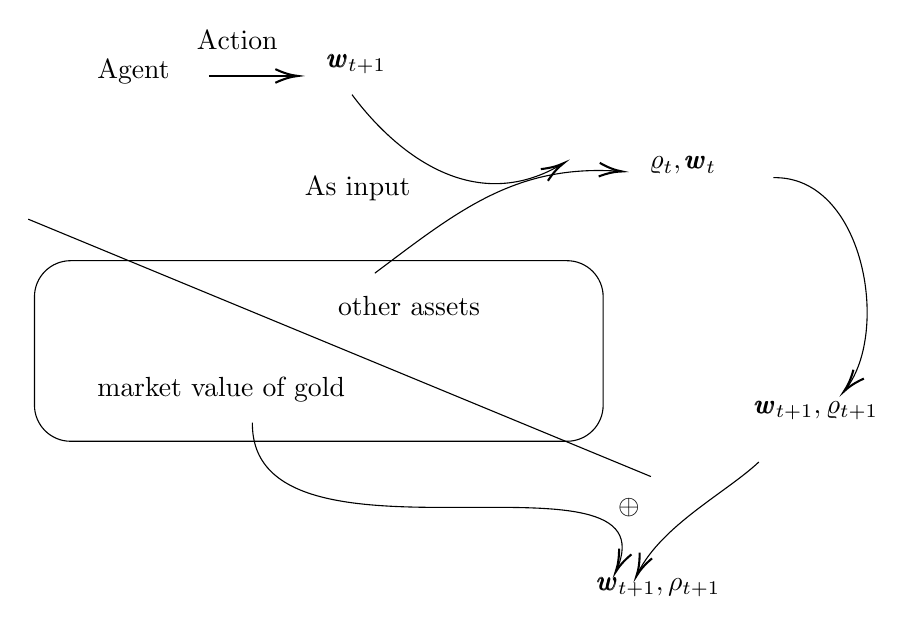
\begin{tikzpicture}[x=0.75pt,y=0.75pt,yscale=-1,xscale=1]
%uncomment if require: \path (0,300); %set diagram left start at 0, and has height of 300

%Rounded Rect [id:dp8834591968202742]
\draw   (100,133.4) .. controls (100,123.79) and (107.79,116) .. (117.4,116) -- (356.6,116) .. controls (366.21,116) and (374,123.79) .. (374,133.4) -- (374,185.6) .. controls (374,195.21) and (366.21,203) .. (356.6,203) -- (117.4,203) .. controls (107.79,203) and (100,195.21) .. (100,185.6) -- cycle ;
%Straight Lines [id:da7362281283591992]
\draw    (97,96) -- (397,220) ;
%Curve Lines [id:da160010014065319]
\draw    (264,122) .. controls (303.6,92.3) and (331.44,69.46) .. (381.48,72.89) ;
\draw [shift={(383,73)}, rotate = 184.48] [color={rgb, 255:red, 0; green, 0; blue, 0 }  ][line width=0.75]    (10.93,-3.29) .. controls (6.95,-1.4) and (3.31,-0.3) .. (0,0) .. controls (3.31,0.3) and (6.95,1.4) .. (10.93,3.29)   ;
%Straight Lines [id:da7831526497431593]
\draw    (184,27) -- (225,27) ;
\draw [shift={(227,27)}, rotate = 180] [color={rgb, 255:red, 0; green, 0; blue, 0 }  ][line width=0.75]    (10.93,-3.29) .. controls (6.95,-1.4) and (3.31,-0.3) .. (0,0) .. controls (3.31,0.3) and (6.95,1.4) .. (10.93,3.29)   ;
%Curve Lines [id:da06593268260339469]
\draw    (253,36) .. controls (269.83,58.77) and (308.22,96.24) .. (353.62,69.82) ;
\draw [shift={(355,69)}, rotate = 148.67] [color={rgb, 255:red, 0; green, 0; blue, 0 }  ][line width=0.75]    (10.93,-3.29) .. controls (6.95,-1.4) and (3.31,-0.3) .. (0,0) .. controls (3.31,0.3) and (6.95,1.4) .. (10.93,3.29)   ;
%Curve Lines [id:da8174394958071393]
\draw    (456,76) .. controls (499.34,75.02) and (512.6,149.71) .. (491.01,177.75) ;
\draw [shift={(490,179)}, rotate = 310.43] [color={rgb, 255:red, 0; green, 0; blue, 0 }  ][line width=0.75]    (10.93,-3.29) .. controls (6.95,-1.4) and (3.31,-0.3) .. (0,0) .. controls (3.31,0.3) and (6.95,1.4) .. (10.93,3.29)   ;
%Curve Lines [id:da327303584584819]
\draw    (205,194) .. controls (204.01,272.61) and (408.94,200.73) .. (380.45,265.02) ;
\draw [shift={(380,266)}, rotate = 295.16] [color={rgb, 255:red, 0; green, 0; blue, 0 }  ][line width=0.75]    (10.93,-3.29) .. controls (6.95,-1.4) and (3.31,-0.3) .. (0,0) .. controls (3.31,0.3) and (6.95,1.4) .. (10.93,3.29)   ;
%Curve Lines [id:da9374685353653947]
\draw    (449,213) .. controls (433.4,227.63) and (402.59,243.2) .. (390.86,266.21) ;
\draw [shift={(390,268)}, rotate = 294.62] [color={rgb, 255:red, 0; green, 0; blue, 0 }  ][line width=0.75]    (10.93,-3.29) .. controls (6.95,-1.4) and (3.31,-0.3) .. (0,0) .. controls (3.31,0.3) and (6.95,1.4) .. (10.93,3.29)   ;

% Text Node
\draw (129,171) node [anchor=north west][inner sep=0.75pt]   [align=left] {market value of gold};
% Text Node
\draw (245,132) node [anchor=north west][inner sep=0.75pt]   [align=left] {other assets};
% Text Node
\draw (395,64.4) node [anchor=north west][inner sep=0.75pt]    {$\varrho _{t} ,\pmb{w}_{t}$};
% Text Node
\draw (129,18) node [anchor=north west][inner sep=0.75pt]   [align=left] {Agent};
% Text Node
\draw (240,15.4) node [anchor=north west][inner sep=0.75pt]    {$\pmb{w}_{t + 1}$};
% Text Node
\draw (446,182.4) node [anchor=north west][inner sep=0.75pt]    {$\pmb{w}_{t+1} , \varrho _{t+1}$};
% Text Node
\draw (177,4) node [anchor=north west][inner sep=0.75pt]   [align=left] {Action};
% Text Node
\draw (229,74) node [anchor=north west][inner sep=0.75pt]   [align=left] {As input};
% Text Node
\draw (380,229.4) node [anchor=north west][inner sep=0.75pt]    {$\oplus $};
% Text Node
\draw (370,267.4) node [anchor=north west][inner sep=0.75pt]    {$\pmb{w}_{t+1}, \rho_{t+1} $};

\end{tikzpicture}
\caption{No gold trade workflow}
\label{fig:no_gold}
\end{figure}

\subsubsection{The observation}

% 在强化学习概念中,observation是神经网络对环境的认知术语。在我们的模型中,我们将observation设定为标准化的前$n$天价格矩阵,以及目前拥有的资产分布情况,即$\pmb{w}$

In reinforcement learning concepts, observation is the cognitive term for a neural network's environment. In our model, we set the observation to be the normalized price matrix of the previous $n$ days, and the distribution of assets currently owned, i.e. $\pmb{w}$.

% 之所以给模型输入$\pmb{w}$是因为一个良好的agent应该知道他在某一个时间刻拥有多少的资产比例。如果agent希望习得根据transaction cost的变化而改变交易次数,也就是变得交易谨慎,他必须要学习什么输出$\pmb{w}$是“不交易的”,输入$\pmb{w}$可以使模型更快地收敛。

The reason for entering $\pmb{w}$ into the model is because a good agent should know what proportion of assets it has at a given moment. If the agent wants to learn to change the number of transactions according to the change of transaction cost, that is, to become transaction prudent, he must learn what output $\pmb{w}$ is ``no transaction'', enter $\pmb{w}$ can make the model converge faster.

\begin{figure}[h]
\centering
 %set default line width to 0.75pt
\scalebox{0.9}[0.9]{
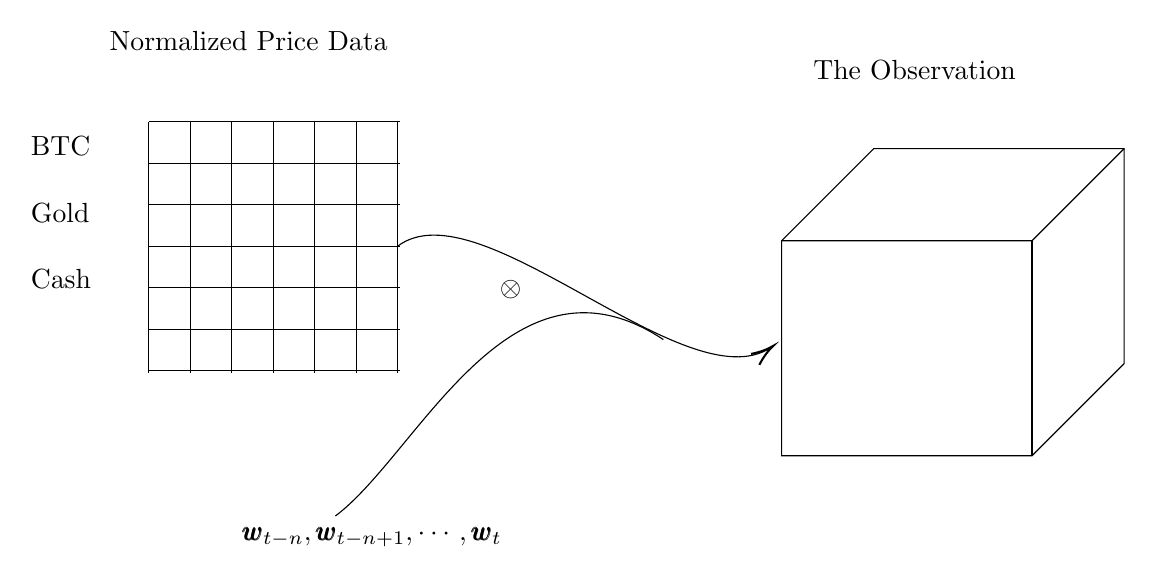
\begin{tikzpicture}[x=0.75pt,y=0.75pt,yscale=-1,xscale=1]
  %uncomment if require: \path (0,300); %set diagram left start at 0, and has height of 300

  %Shape: Cube [id:dp0031259884345929967]
  \draw   (391,124.4) -- (435.4,80) -- (556,80) -- (556,183.6) -- (511.6,228) -- (391,228) -- cycle ; \draw   (556,80) -- (511.6,124.4) -- (391,124.4) ; \draw   (511.6,124.4) -- (511.6,228) ;
  %Shape: Grid [id:dp3629674359367516]
  \draw  [draw opacity=0] (86,67) -- (207,67) -- (207,188) -- (86,188) -- cycle ; \draw   (86,67) -- (86,188)(106,67) -- (106,188)(126,67) -- (126,188)(146,67) -- (146,188)(166,67) -- (166,188)(186,67) -- (186,188)(206,67) -- (206,188) ; \draw   (86,67) -- (207,67)(86,87) -- (207,87)(86,107) -- (207,107)(86,127) -- (207,127)(86,147) -- (207,147)(86,167) -- (207,167)(86,187) -- (207,187) ; \draw    ;
  %Curve Lines [id:da9295803655851189]
  \draw    (206,127) .. controls (245.6,97.3) and (344.99,202.85) .. (385.78,175.86) ;
  \draw [shift={(387,175)}, rotate = 143.13] [color={rgb, 255:red, 0; green, 0; blue, 0 }  ][line width=0.75]    (10.93,-3.29) .. controls (6.95,-1.4) and (3.31,-0.3) .. (0,0) .. controls (3.31,0.3) and (6.95,1.4) .. (10.93,3.29)   ;
  %Curve Lines [id:da9533332638936705]
  \draw    (176,257) .. controls (216,227) and (260,123) .. (334,172) ;

  % Text Node
  \draw (405,36) node [anchor=north west][inner sep=0.75pt]   [align=left] {The Observation};
  % Text Node
  \draw (66,22) node [anchor=north west][inner sep=0.75pt]   [align=left] {Normalized Price Data};
  % Text Node
  \draw (130,261.4) node [anchor=north west][inner sep=0.75pt]    {$\pmb{w}_{t-n}, \pmb{w}_{t-n+1}, \cdots, \pmb{w}_t$};
  % Text Node
  \draw (254,142.4) node [anchor=north west][inner sep=0.75pt]    {$\otimes $};
  % Text Node
  \draw (28,73) node [anchor=north west][inner sep=0.75pt]   [align=left] {BTC\\\\Gold\\\\Cash};


  \end{tikzpicture}
}
\caption{The building process of observation arrays}
\end{figure}


\subsubsection{Risk Constraint \label{risk-constraint}}

% 风险约束是决定交易发生与否的重要方式。如前文所定义,市场风险溢价RP代表了一次交易在有风险的情况下多获得的收益(相比于无风险的情况而言)。更大的RP通常意味着更多的收益,同时也会带来更大的风险(It provides a quantitative measure of the extra return demanded by market participants for the increased risk.)。RP的数学公式:

Risk constraint is an important way of deciding whether a transaction occurs or not.
As we have mentioned before, the \textit{market risk premium} shows the extra expected return on a market portfolio than on the risk-free rate \cite{duarte2015equity}.
It provides a quantitative measure of the extra return demanded by market participants for the increased risk.
The formula for RP is

\begin{equation}
  RP = E(r_m) - r_f,
\end{equation}

where $E(r_m)$ stands for the expected return rate on a market portfolio, and $r_f$ is the return rate on a risk-free rate.
$E(r_m)$ is obtained from the actual market performance, or in our model,
from the algorithm outputs.

% 通过人为为RP设置一个界限的方法,可以改变agent的策略。这个界限代表着交易与否的分界。当RP小于该界限时允许进行交易,而RP大于该界限时不允许进行交易,这样来进一步达到提高收入与降低风险这两个目标。而针对它们优先级的不同,可以为RP设置不同的界限:当提高收入更为重要时,界限设置得较大,允许agent进行风险较高的交易;当降低风险更为重要时,界限设置的较小,以回避可能带来的不确定性。

The agent's strategy can be changed by artificially setting a cut-off for $RP$,
which indicates the boundary between a transaction occuring and the opposite.
Transactions are allowed when the RP is less than this cut-off and not allowed when the RP is greater than it, thus furthering the twin objectives of maximizing the profit and minimizing the risk.
Different cut-offs can be set for RP depending on their priority: when maximizing profit is more important, the cut-off is set higher to allow agent to undertake riskier transactions; when reducing risk is more important, the cut-off is set lower to avoid the uncertainty that may arise.

% 同时,更新w的算法得到进一步简化。当交易不被允许时,w(t+1)直接继承w(t)即可。
% 这个好像没必要说,和这一部分关系不大

\subsection{The Model Results}

Figure \ref{RL-Results}  plots the total value of all assets against time,
respectively using Proximal policy optimization(PPO), RNN-LSTM and Autoregression model.

\begin{figure}[h]
  \small
  \centering
  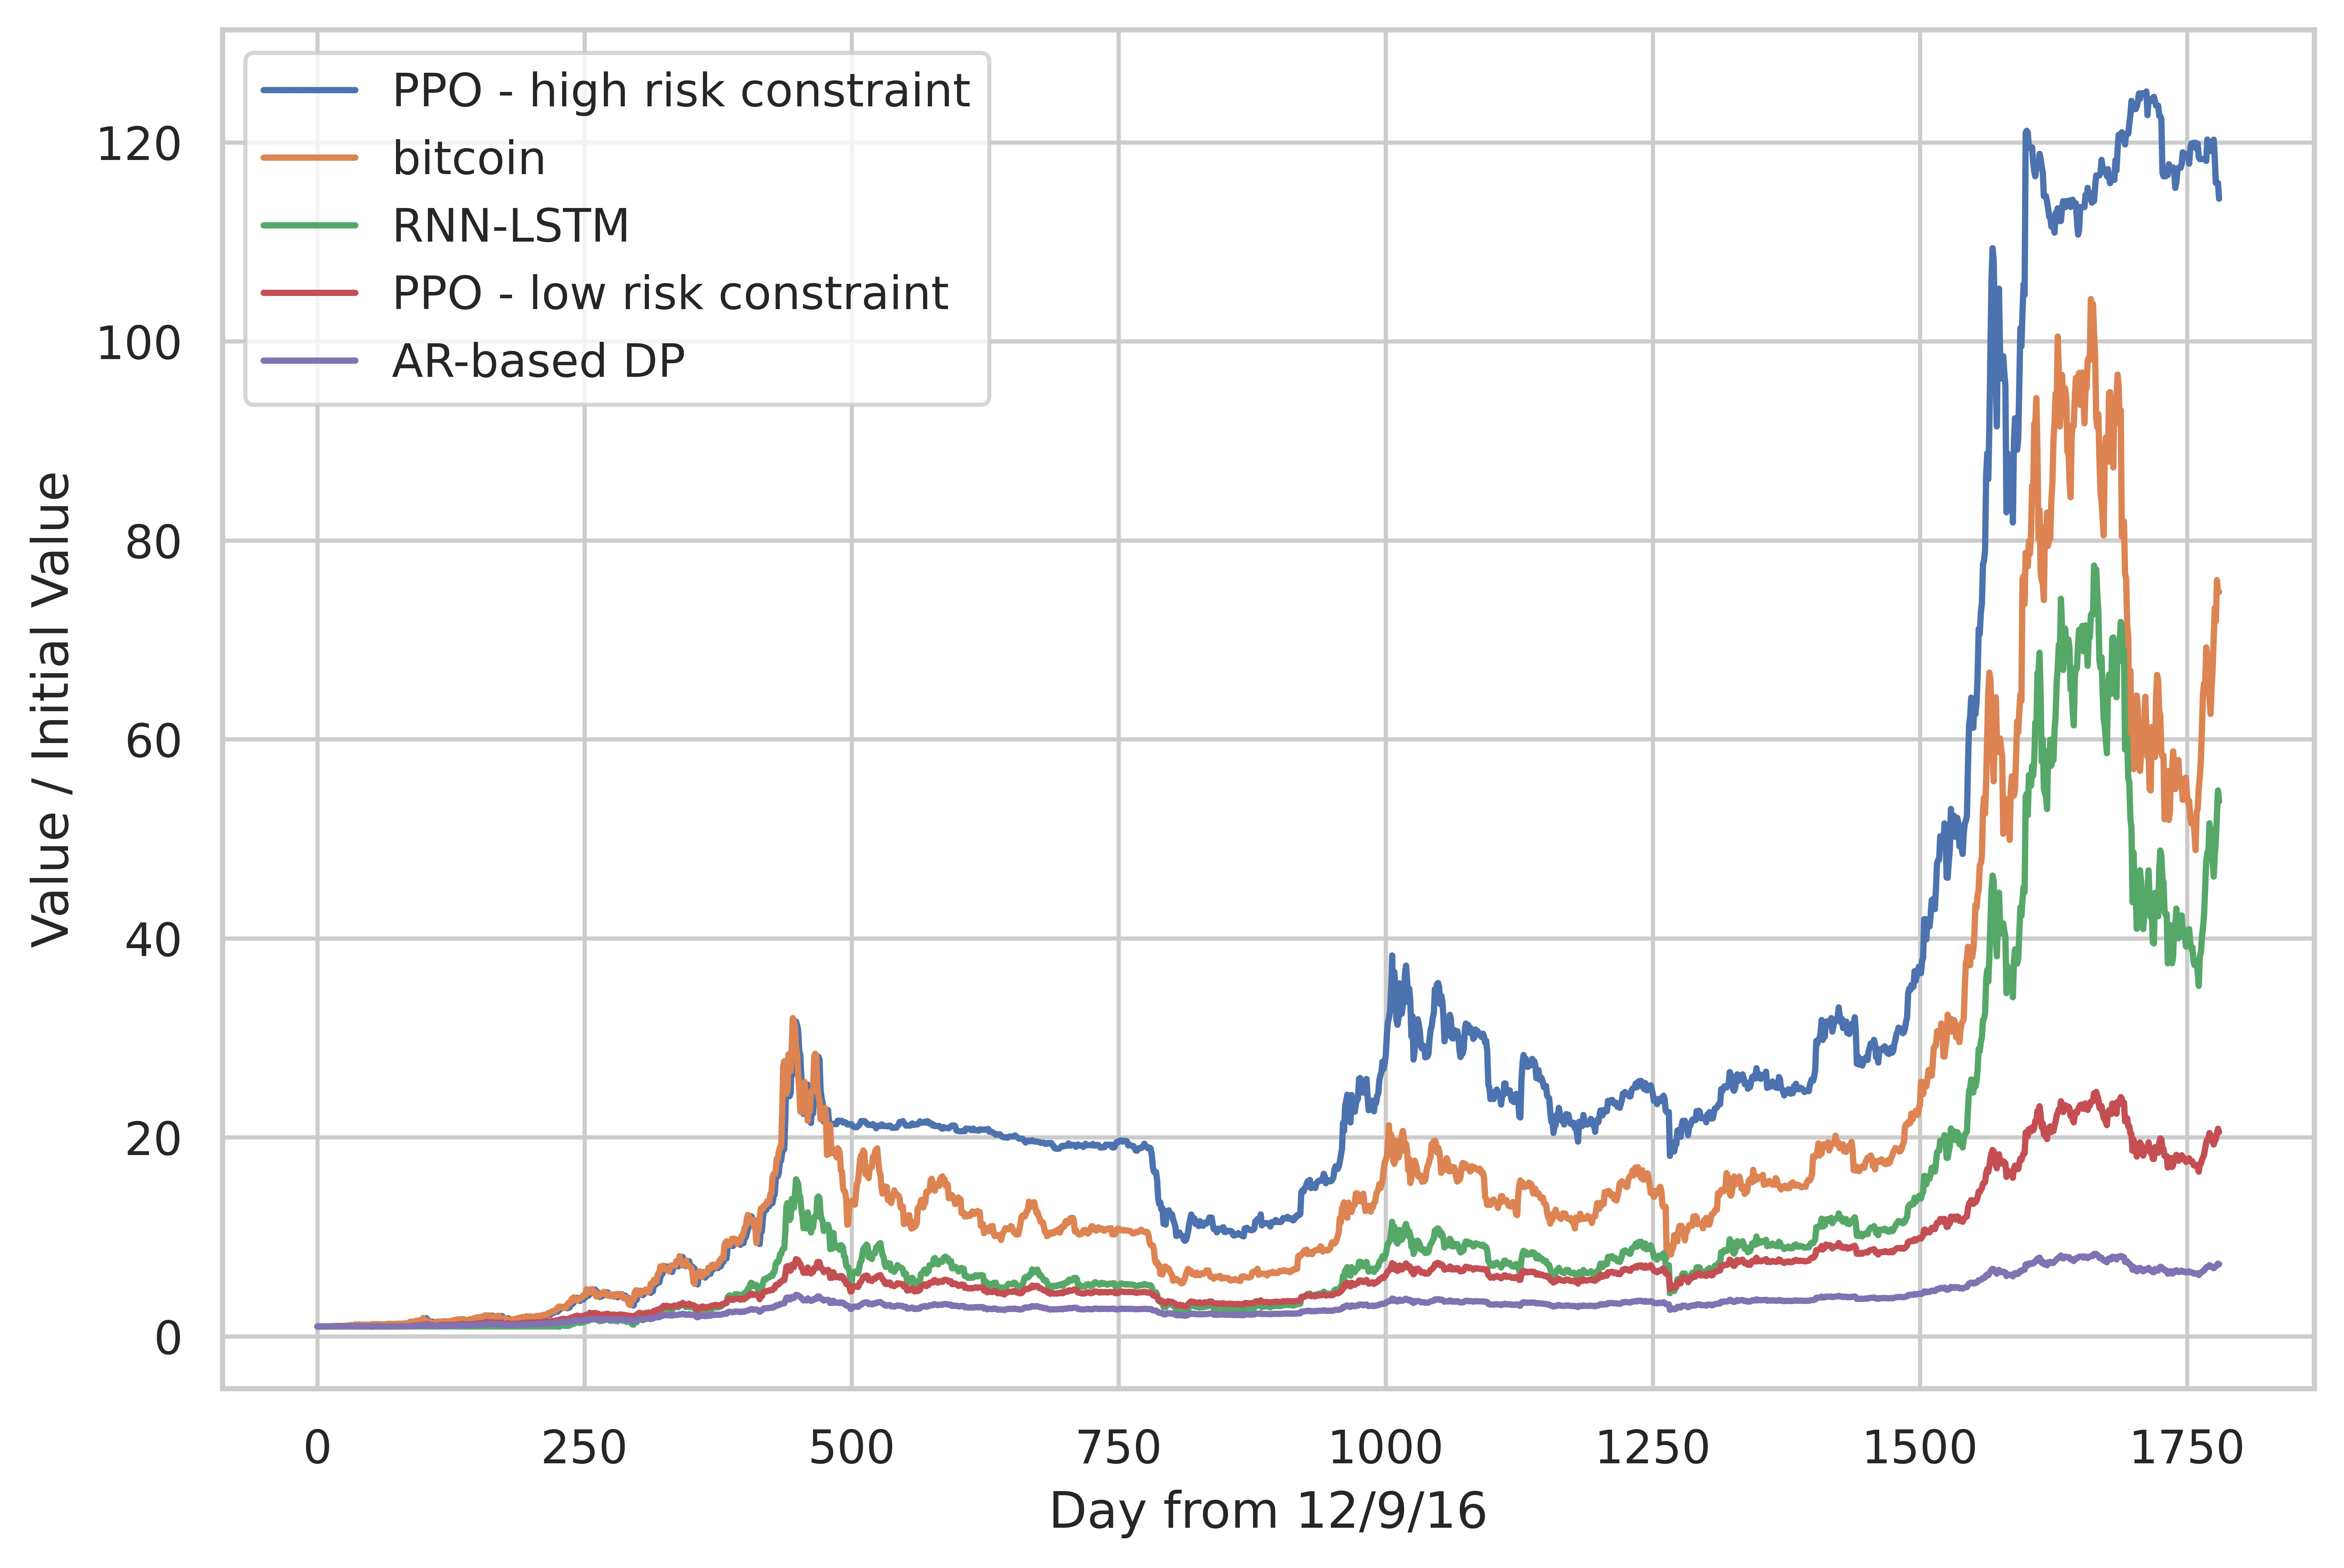
\includegraphics[width=10cm]{RL-final.jpg}
  \caption{Reinforcement learning results} \label{RL-Results}
\end{figure}

Proximal policy optimization with high risk constraint works the best among all the algorithms, with an acceptable amount of risk and high profit. PPO with low risk constraint works well when control of risk is a priority, with smaller but consistently growing returns that are less affected by the price of bitcoin. Both RNN-LSTM and Autoregression model performed relatively poorly, with the former being too risky and the latter too low rewarding.

The actions made the agent in the face of changes in the price of Bitcoin have a significant impact on its outcome.
Figure \ref{BTC} shows the number of \textit{units} of bitcoin bought by the agent against price changes in bitcoin with the PPO algorithm.

\begin{figure}[h]
  \small
  \centering
  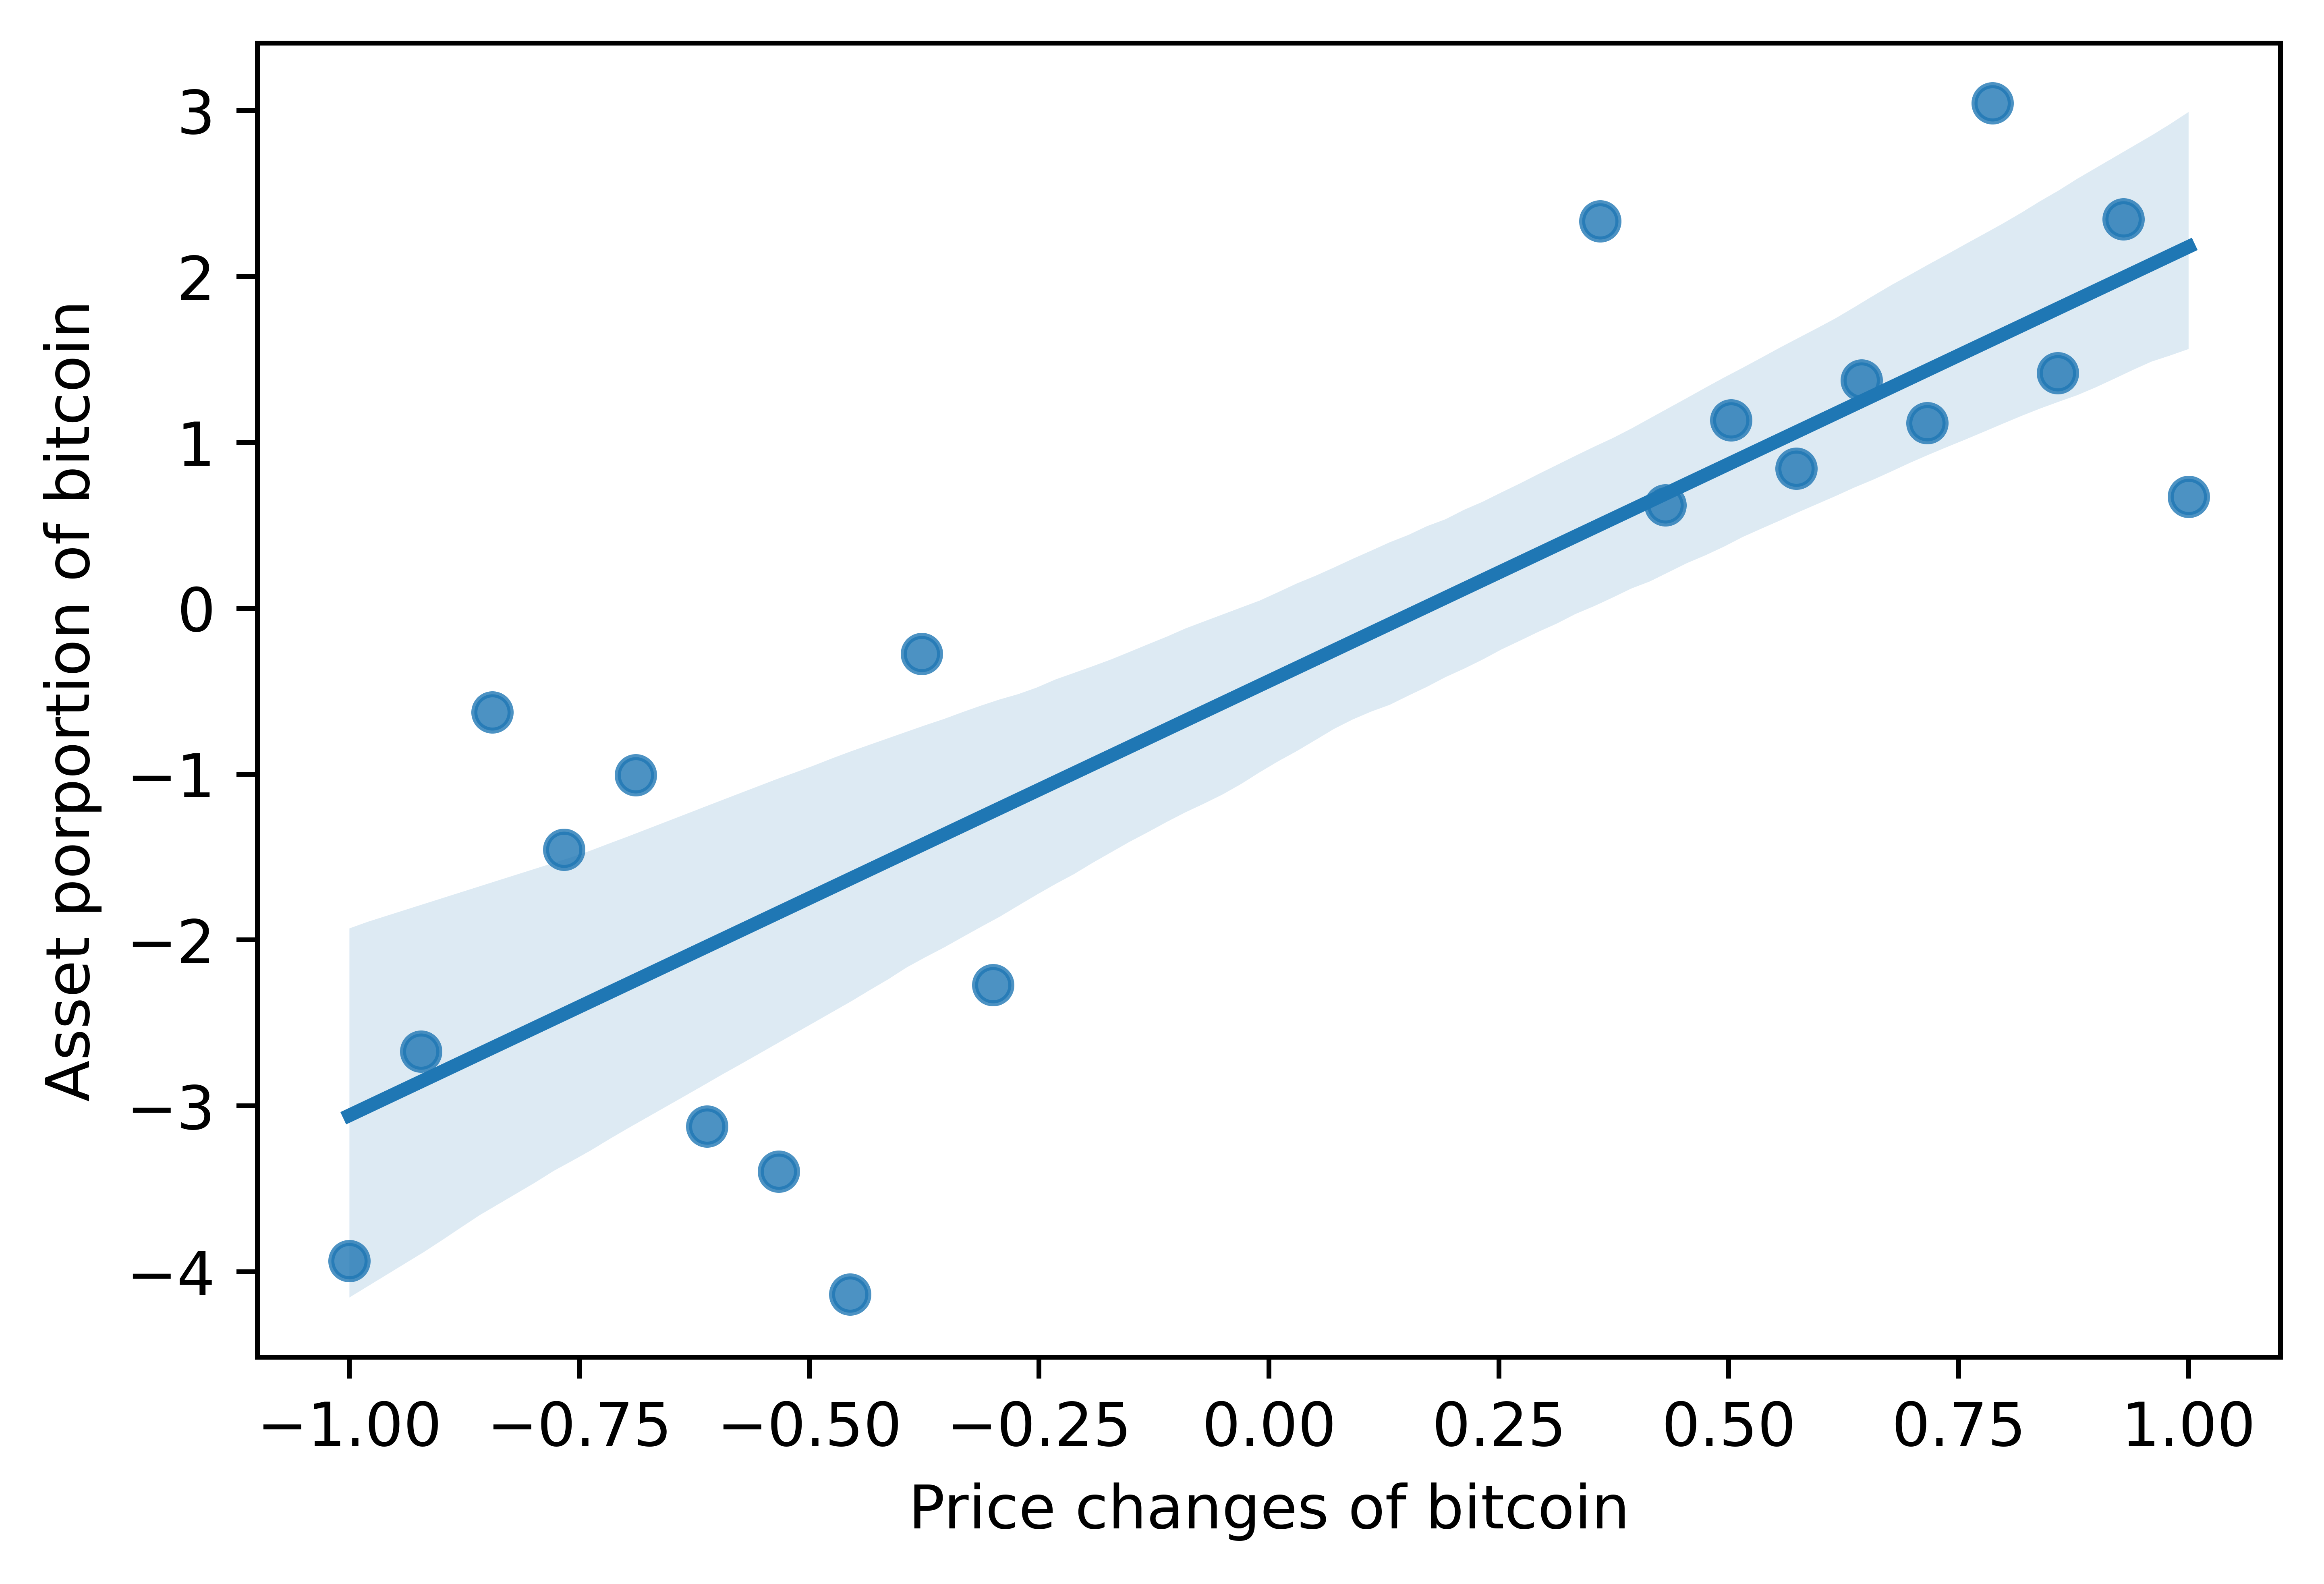
\includegraphics[width=10cm]{linear.png}
  \caption{Agent behavior against price changes of BTC} \label{BTC}
\end{figure}

Each point in the figure stands for one actual transaction made by the agent.
The x-axis represents the average changes in price in the next 15 days.
The y-axis represents the amount of purchases, with positive and negative values indicating buys and sells respectively.
When the agent believes that there will be a significant change in the price of Bitcoin, it will change its holdings accordingly.
As can be seen from the figure, the purchase volume and change in price can be approximately fitted into a positive correlation relationship.

And finally, the value of the initial \$1,000 is shown in table \ref{final-value}:

\begin{table}[h]
  \centering
  \begin{tabular}{@{}lr@{}}
    \toprule
    Algorithm & Final value(\$) \\
    \midrule
    Proximal policy optimization (high-risk) & 112,630 \\
    {\color{gray} All in bitcoin} & {\color{gray} 76,120} \\
    RNN-LSTM & 55,350 \\
    Proximal policy optimization (low-risk) & 21,450 \\
    AR-based DP & 8,040 \\
    \bottomrule
  \end{tabular}
  \caption{Final value of funds}
  \label{final-value}
\end{table}

\subsection{Transactions cost sensitivity}

As mentioned in the hypothesis section, transaction cost highly affects the decision-making process and the final result of the algorithm.
A higher transaction cost means more losses with equal transaction amounts,
leading to negative rewards given to the agent.
The agent will try to lower these losses, by the means of decreasing total transaction amount.
This can be done by reducing rather the amount per trade or the times of transaction.
Figure \ref{Transaction-cost} shows the transaction count of bitcoin against its transaction cost.
With the percentage of transaction cost increasing, the agent significantly reduces the number of transactions.

\begin{figure}[h]
  \small
  \centering
  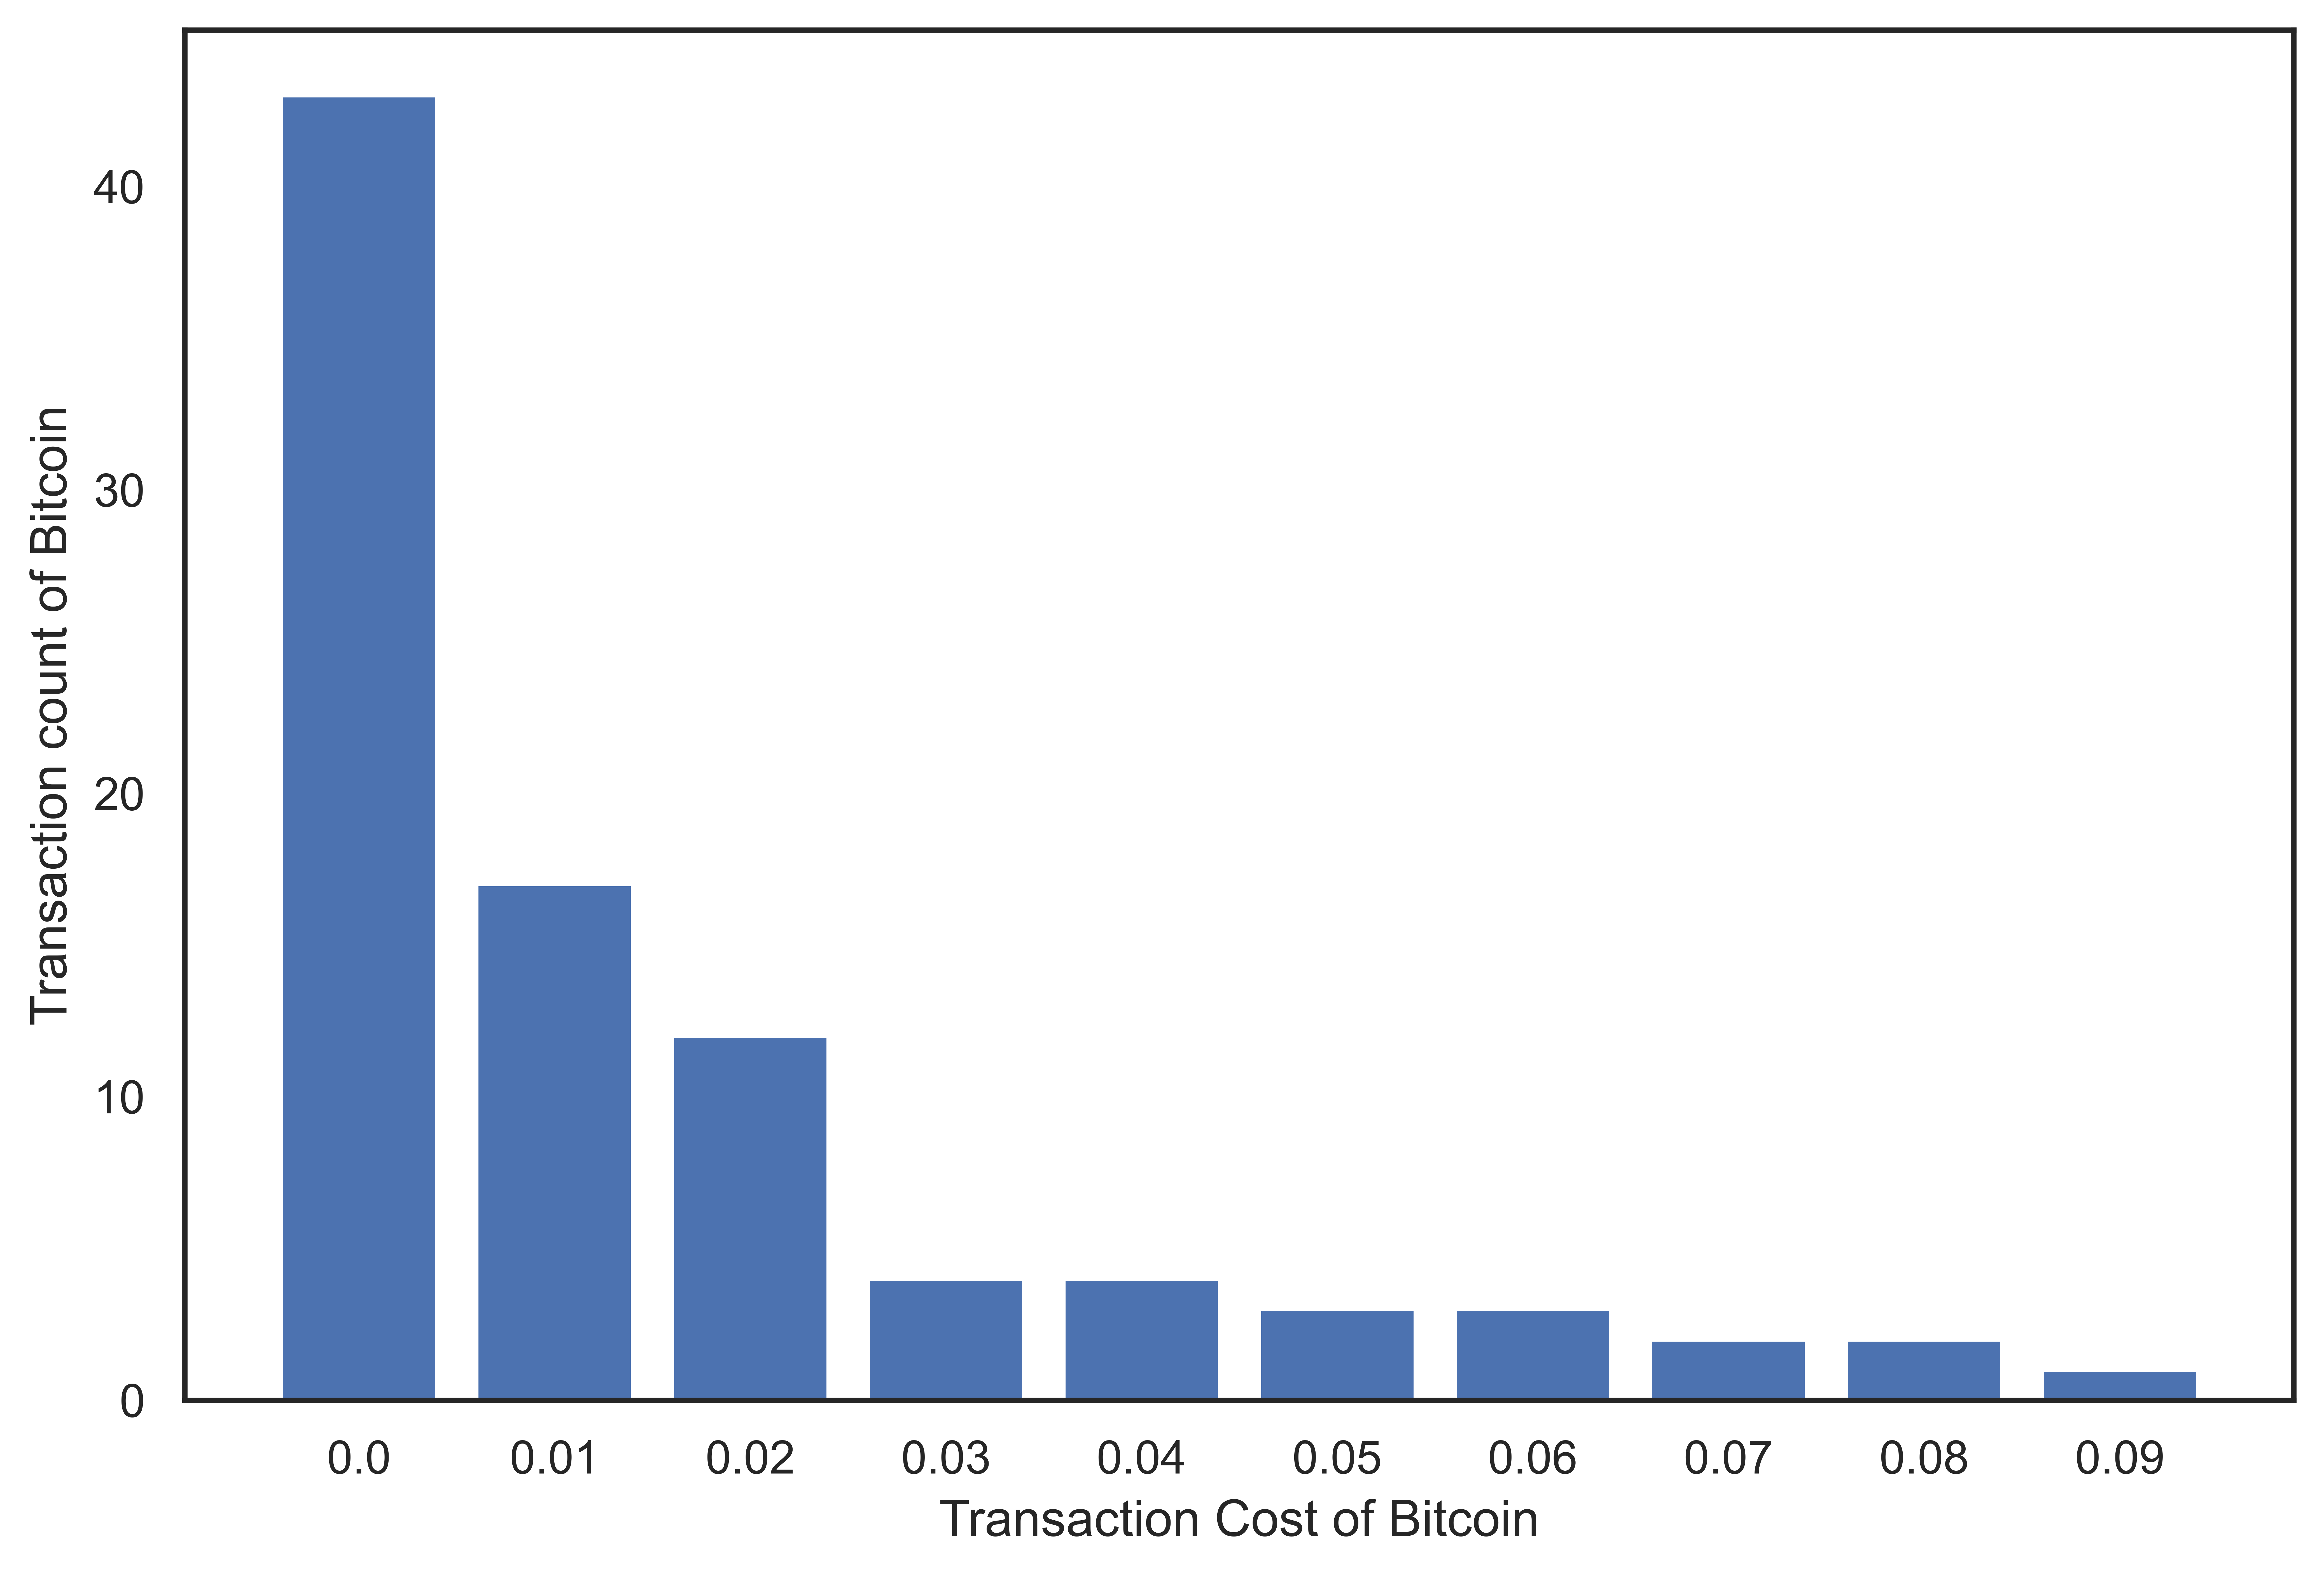
\includegraphics[width=11cm]{Transaction-cost.png}
  \caption{Transaction count against the transaction cost of BTC}
  \label{Transaction-cost}
\end{figure}

\section{Conclusions}

This paper presents an automatic portfolio management model.
Among all the algorithms used in the article, the method of reinforcement learning with the proximal policy optimization works the best.
The agent's strategy in PPO changes for different risk constraints.
With a relatively high risk constraint, the agent performs a high-risk strategy and raises total assets to 112 times, in the 5-year trading period.
With a low risk constraint, the agent gained 21 times of return. Although lower, the returns of the latter are more stable and have largely been on an upward trend over the five-year period.

As for the transaction cost sensitivity, our agent significantly reduces its number of trades as the transaction cost rising, to reduce the loss of reward in the trades.

\section{Strengths and weaknesses}

\subsection{Strengths}
\begin{itemize}
\item \textbf{Controlable risk constraint}\\
By setting different cut-offs for the risk premium, we can artificially adjust the behaviour of agents and thus the relationship between return and risk. This incorporates the idea of supervised-learning into reinforcement learning and makes our model applicable to market traders with different objectives.
\item \textbf{End-to-end learning and planning}\\
The end-to-end PPO algorithm is more accurate than the multi-staged algorithm, considering the fact that it combines multiple steps and eliminates the effects between them.
\item \textbf{Appliable for different assets}\\
This model does not only apply for the transactions of bitcoin and gold.
It can also be used to forecast and plan the distribution of other types of assets such as stocks and shares.
\end{itemize}

\subsection{Weaknesses}
\begin{itemize}
  \item \textbf{Relatively long learning process}\\
  The end-to-end PPO algorithm consumes more resources and takes longer compared to two-staged methods.
  In our case, the model took one hour to train to get better results, while two-staged models tend to converge quickly.
  \item \textbf{Reliance on substantial historical data}\\
  The PPO algorithm relies more on historical data than some of the other algorithms such as VAR. This means that it does not perform well in cases where there is less historical data.
\end{itemize}

% \begin{thebibliography}{99}
% \bibitem{1} D.~E. KNUTH   The \TeX{}book  the American
% Mathematical Society and Addison-Wesley
% Publishing Company , 1984-1986.
% \bibitem{2}Lamport, Leslie,  \LaTeX{}: `` A Document Preparation System '',
% Addison-Wesley Publishing Company, 1986.
% \bibitem{3}\url{https://www.latexstudio.net/}
% \end{thebibliography}

\bibliographystyle{unsrt} %规定了参考文献的格式
\begin{center}
\bibliography{reference} %调出LaTeX生成参考文献列表
\end{center}

\newpage
% Generate the Memorandum, if it's needed.
\addcontentsline{toc}{section}{Memorandum}
\memoto{Trader}
\memofrom{MCM team 2207690}
\memosubject{An automated trade decision-making model for Bitcoin and gold}
\memodate{\today}
\begin{memo}[Memorandum]
  \lipsum[1-3]
\end{memo}

% \begin{appendices}

% \section{First appendix}

% In addition, your report must include a letter to the Chief Financial Officer (CFO) of the Goodgrant Foundation, Mr. Alpha Chiang, that describes the optimal investment strategy, your modeling approach and major results, and a brief discussion of your proposed concept of a return-on-investment (ROI). This letter should be no more than two pages in length.

% \begin{letter}{Dear, Mr. Alpha Chiang}

% \lipsum[1-2]

% \vspace{\parskip}

% Sincerely yours,

% Your friends

% \end{letter}
% Here are simulation programmes we used in our model as follow.\\

% \textbf{\textcolor[rgb]{0.98,0.00,0.00}{Input matlab source:}}
% \lstinputlisting[language=Matlab]{./code/mcmthesis-matlab1.m}

% \section{Second appendix}

% some more text \textcolor[rgb]{0.98,0.00,0.00}{\textbf{Input C++ source:}}
% \lstinputlisting[language=C++]{./code/mcmthesis-sudoku.cpp}

% \lstinputlisting[language=python]{./code/Harbin.py}

% \section{Third appendix}

% When you need to insert a table, use this template.

% \begin{table}
% \centering
% \begin{tabular}{@{}lr@{}}
%   \toprule
%   Algorithm & Final value(\$) \\
%   \midrule
%   Proximal policy optimization (high risk) & 112 \\
%   {\color{gray} All in bitcoin} & {\color{gray} 76} \\
%   RNN-LSTM & 55 \\
%   Proximal policy optimization (low risk) & 21 \\
%   AR-based DP & 8 \\
%   \bottomrule
% \end{tabular}
% \caption{Final value of funds}
% \label{final-value123}
% \end{table}

% \end{appendices}

\end{document}

%%
%% This work consists of these files mcmthesis.dtx,
%%                                   figures/ and
%%                                   code/,
%% and the derived files             mcmthesis.cls,
%%                                   mcmthesis-demo.tex,
%%                                   README,
%%                                   LICENSE,
%%                                   mcmthesis.pdf and
%%                                   mcmthesis-demo.pdf.
%%
%% End of file `mcmthesis-demo.tex'.

